%%%%%%%%%%%%%%%%%%%%%%%%%%%%%%%%%%%%%%%%%%%%%%%%%%%%%%%%%%%%%%%%%%%%%%%%%%%%%
% 1- INICIALITZACIÓ
%%%%%%%%%%%%%%%%%%%%%%%%%%%%%%%%%%%%%%%%%%%%%%%%%%%%%%%%%%%%%%%%%%%%%%%%%%%%%

\documentclass[catalan,final]{../latex-manual-template/manual_template}

% Loading packages
% ALL NEEDED PACKAGES ARE LOADED HERE


% Generate English ordinal numbers
\usepackage[super]{nth}

% Improved citation handling in LaTeX
\usepackage[sort,nocompress]{cite}

% Graphic elemens 
\usepackage{tikz}

\usetikzlibrary{shapes.geometric, arrows}
\usetikzlibrary{trees}
\usetikzlibrary{shadows}

\tikzstyle{startstop} = [rectangle, rounded corners, minimum width=3cm, minimum height=1cm,text centered, text width=3cm, draw=black, fill=white]
\tikzstyle{io} = [trapezium, trapezium left angle=70, trapezium right angle=110, minimum width=3cm, minimum height=1cm, text centered, text width=2.8cm , draw=black, fill=white]
\tikzstyle{process} = [rectangle, minimum width=3cm, minimum height=1cm, text centered, text width=3cm, draw=black, fill=white]
\tikzstyle{decision} = [diamond, minimum width=2cm, minimum height=1cm, text centered, text width=2cm, draw=black, fill=white]
\tikzstyle{arrow} = [thick,->,>=stealth]

% Use existing qtree syntax for trees in TikZ
\usepackage{tikz-qtree} % Tree diagram

% Draw electrical networks with TikZ
\usepackage{circuitikz} % Electrical circuits

% Control layout of itemize, enumerate, description
\usepackage{enumitem}   % Introduce lists of items

% Customising captions in floating environments
\usepackage[font={small,it},labelfont=bf]{caption}

% Improved interface for floating objects
\usepackage{float}

% Deprecated: Figures divided into subfigures
\usepackage{subfigure}

% Colour control for LaTeX documents / Add colour to LaTeX tables
\usepackage{color, colortbl}

%  A variable-width \parbox command
\usepackage{pbox}

% Access bold symbols in maths mode
\usepackage{bm} % Provide bold maths symbols

% Enhanced support for graphics
\usepackage{graphicx}
\graphicspath{/images/}
\addtolength{\footnotesep}{1mm} % change to 1mm
\interfootnotelinepenalty=10000 % Avoid to break a footnote into two different pages


%% * OPCIONS A CONFIGURAR al \documentclass
%%    - Estat del document: final o draft
%%      NOTA: Draft no inserta les figures i marca només l'espai que
%%      ocupen. També s'indica quan el text sobrepassa els marges.
%%      Draft és molt útil per compilar ràpid el document si no és important
%%      en aquell moment visualitzar les figures.
%%    - Idioma PRINCIPAL del document: catalan, spanish, english, french...

% Multilingual support for LaTeX, LuaLaTeX, XeLaTeX, and Plain TeX
\usepackage[english]{babel}

%%    NOTA: per canviar d'idioma al mig del document usar:
%%          \selectlanguage{nom_idioma}
%%%%%%%%%%%%%%%%%%%%%%%%%%%%%%%%%%%%%%%%%%%%%%%%%%%%%%%%%%%%%%%%%%%%%%%%%%%%%

%%%%%%%%%%%%%%%%%%%%%%%%%%%%%%%%%%%%%%%%%%%%%%%%%%%%%%%%%%%%%%%%%%%%%%%%%%%%%
% 2- CÀRREGA DE PAQUETS ADICIONALS (OPCIONALS)
%%%%%%%%%%%%%%%%%%%%%%%%%%%%%%%%%%%%%%%%%%%%%%%%%%%%%%%%%%%%%%%%%%%%%%%%%%%%%

% Accept different input encodings
\usepackage[utf8]{inputenc}
\DeclareUnicodeCharacter{00A0}{ }

% Mathematical symbols of American Mathematical Society  
\usepackage{amssymb, amsmath, amsfonts}

% Extending the array and tabular environments
\usepackage{array}                      %% El paquet array proporciona eines molt útils a l'hora de fer equacions amb matrius       

% Create tabular cells spanning multiple rows
\usepackage{multirow}                   %% Paquet que permet fer taules fusionant cel·les de files consecutives          

% Allow tables to flow over page boundaries
\usepackage{longtable}                  %% Paquet molt útil en cas de tenir taules molt llargues que ocupin vàries pàgines          

% Numbered cases environment
\usepackage{cases}                      % Two different labeled equations (warning: tiene que ir detras de 'ansmath')

% Permit footnotes in tables
\usepackage{tablefootnote}

% Include PDF documents in LaTeX
\usepackage{pdfpages}

% Easily include nicely syntax highlighted m-code in your LaTeX documents
\usepackage[framed,numbered,autolinebreaks,useliterate]{mcode}


%% Paquet molt útil que permet activar links en el PDF final.
%% * NO OBLIDAR DE CONFIGURAR els quatre primer camps!
% Extensive support for hypertext in LaTeX
\usepackage[
  pdfauthor={Nom Cognoms autor},            % Configurar adientment
  %pdftitle={Treball Fi de Carrera - autor}, % Configurar adientment
  %pdfsubject={Titol del TFC aqui},          % Configurar adientment
  % Modificació respecte a la versió 2.1 - Iván Padilla Montero - Juliol 2014
  pdftitle={Treball Fi de Grau - autor}, % Configurar adientment
  pdfsubject={Titol del TFG aqui},          % Configurar adientment  
  pdfkeywords={keyword1, keyword2, ...},    % Configurar adientment
  pdfcreator={EETAC-UPC}, 
  pdfproducer={LaTeX, dvipdf},
  pdfdisplaydoctitle=true, plainpages=false, linktocpage=true,         
  colorlinks=true, linkcolor=blue,citecolor=blue,urlcolor=blue,
  hyperfootnotes=false, pagebackref=true, pdfpagelabels=true,            % PARA NO PONER NUMERO DE PAGINA EN LA REFERENCIA
  pdfpagemode=UseOutlines,
]{hyperref}
%% NOTA IMPORTANT!:
%% Per tal que hyperef funcioni correctament amb els capitols o seccions no
%% numerats (\chapter*{}), com per exemple introducció, conclusions i bibliografia
%% cal posar les dues comandes seguents ABANS del \chapter*{} en questió


% View the layout of a document
\usepackage{layout}

% Draw a page-layout diagram
\usepackage{showframe}

% Graphics package-alike macros for “general” boxes
\usepackage[export]{adjustbox}


%% Permet arranjar matricialment multiples figures
%% NOTA: afegir aquest paquet DESPRES del hyperref!!
%%       Si no es desitja utilitzar aquest paquet, comentar la linia seguent
%%       i anar TAMBE al fitxer de classe (eetac_tfc_pfc.cls) per substituir: 
%%       \RequirePackage[subfigure]{tocloft}  per  \RequirePackage{tocloft}
% Automates layout when using the subfigure package
\usepackage{subfigmat}     



% UNUSED

% \usepackage{mwe}
% \usepackage{subfigure}
% \usepackage{etoolbox}
% \usepackage[labelfont=bf]{caption}
% \usepackage{subfloat}
% \usepackage{subcaption}
% \usepackage{showframe,subcaption}

%% Permet trencar links URL. 
%% Atenció! afegir aquest paquet DESPRES del hyperref!!
%\usepackage{breakurl} 

%%%%%%%%%%%%%%%%%%%%%%%%%%%%%%%%%%%%%%%%%%%%%%%%%%%%%%%%%%%%%%%%%%%%%%%%%%%%%
% 3- DOCUMENT
%%%%%%%%%%%%%%%%%%%%%%%%%%%%%%%%%%%%%%%%%%%%%%%%%%%%%%%%%%%%%%%%%%%%%%%%%%%%%

%%% Configuració de les dades i variables boleanes rellevants del document:
%%%%%%%%%%%%%%%%%%%%%%%%%%%%%%%%%%%%%%%%%%%%%%%%%%%%%%%%%%%%%%%%%%%%%%%%%%%%%
%%%%%%                                                                  %%%%% 
%%%%%%       Fitxer de dades per la memoria TFC/PFC de l'EETAC          %%%%% 
%%%%%%                                                                  %%%%% 
%%%%%%%%%%%%%%%%%%%%%%%%%%%%%%%%%%%%%%%%%%%%%%%%%%%%%%%%%%%%%%%%%%%%%%%%%%%%%


%%%%%%%%%%%%%%%%%%%%%%%%%%%%%%%%%%%%%%%%%%%%%%%%%%%%%%%%%%%%%%%%%%%%%%%%%%%%%%%
%%  VARIABLES A CONFIGURAR                                                  %%%
%%%%%%%%%%%%%%%%%%%%%%%%%%%%%%%%%%%%%%%%%%%%%%%%%%%%%%%%%%%%%%%%%%%%%%%%%%%%%%%

%% - Projecte o Treball de Fi de Carrera?
%%      PFC = true   -> Projecte de Fi de Carrera
%%      PFC = false  -> Treball  de Fi de Carrera
\setboolean{manual}{true}

%% - Escollir la titulació
%\titulacio{Enginyeria Tècnica Aeronàutica, especialitat Aeronavegació}
%\titulacio{Enginyeria T\`ecnica de Telecomunicaci\'o, especialitat Sistemes de Telecomunicaci\'o}
%\titulacio{Enginyeria T\`ecnica de Telecomunicaci\'o, especialitat Telem\`atica}
%\titulacio{Enginyeria de Telecomunicaci\'o (segon cicle)}
% Modificació respecte a la versió 2.1 - Iván Padilla Montero - Juliol 2014
%\titulacio{}
%\titulacio{Grau en Enginyeria d'Aeroports}
%\titulacio{Grau en Enginyeria Telemàtica}
%\titulacio{Grau en Enginyeria de Sistemes de Telecomunicació}


%% - Configurar els idiomes del document
%% Si l'idioma PRINCIPAL del document es l'angles, posar aquesta variable a true
\setboolean{Leng}{false}

%% Escollir entre catala i castella (idioma principial, o nomes pel resum en cas que l'idioma principal sigui anglès)
%%  catala = true   -> idioma principal (o només resum) en Català
%%  catala = false  -> idioma principal (o només resum) en Castella
\setboolean{Lcat}{true}

% Si les dues anteriors variables són falses, es posarà automàticament el títol en castellà
%\setboolean{Les}{false}

%% Titol del document en l'idioma principal del document 
\titol{MANUAL DE MUNTATGE D'UN QUADCOPTER}

%% Titol del document en anglès (Per l'apartat overview)
\titolE{QUADCOPTER DESIGN MANUAL}

%% Titol del document en catala/castella (Per l'apartat resum)
\titolC{MANUAL DE DISSENY I MUNTATGE D'UN QUADCOPTER}
\titolES{MANUAL DE DISEÑO DE UN QUADRICOPTERO}

%% - Nombre d'autors del TFC/PFC?
%%      UNautor = true   Un sol autor
%%      UNautor = false  Més d'un autor
\setboolean{UNautor}{true}

%% - Nom del(s) Autor(s) del document
%% NOTA: En cas de mes d'un autor cal posar la comana \and entre els
%%        noms dels autors
\autor{Llu\´is Hontecillas Guinart}

%% - Nombre de directors del TFC/PFC. Tipicament 1 o 2
%%      UNdirector = true   Un sol director
%%      UNdirector = false  Dos directors
%\setboolean{UNdirector}{true}

%% - Nom del Director del TFC/PFC
%\director{O}




%% - Es vol incloure una dedicatoria?
%%      dedicatoria = true   -> S'afegeix una pagina amb \textDedicatoria
%%      dedicatoria = true   -> No s'afegeix dedicatoria
%% NOTA: no confondre dedicatòria amb agraïments. Una dedicatoria sol ser
%%       un missatge curt d'una o dues frases màxim a la persona, o persones
%%       a les quals es dedica el treball. 
%%       Els agraïments poden ser extensos i l'autor pot agraïr a diverses
%%       persones coses diferents en funció de l'ajuda rebuda, per exemple. 
%%       Si es volen incloure agraïments, fer-ho al fitxer de la 
%%       memòria creant una secció nova amb  \chapter*{Agraïments}
%\setboolean{dedicatoria}{false}
%\textDedicatoria{}

%% - Es vol incloure una pagina d'index de figures?
%\setboolean{paginaLOF}{false}  % List of Figures

%% - Es vol incloure una pagina d'index de taules?
%\setboolean{paginaLOT}{falsa}  % List of Tables 

%% - El projecte ha estat supervisat per alguna persona externa? 
%%   (NOMES en cas de practiques en empresa)
%%      supervisor = true    -> Hi ha un supervisor
%%      supervisor = false   -> No hi ha un supervisor
%\setboolean{supervisor}{false}

%% NOMES en el cas de practiques en empresa (supervisor=true) s'han de 
%% configurar les variables seguents: 

%% Supervisor del TFC/PFC 
%\supervisor{Nom del Supervisor}

%% - Es vol incloure el logotip de l'empresa?
%%   En el cas que el TFC/PFC s'hagi fet en règim d'intercanvi amb una
%%   empresa, es pot afegir el seu logotip a la cantonada superior
%%   dreta de la portada. En aquest cas:
%%   - posar logo=true
%%   - posar el path de la imatge i l'alçada del logo a \mylogo
\setboolean{logo}{false}
\mylogo{./setup/drone_logo.jpg}{3.5cm}
  

%%% Configuració de MACROS o ENTORNS (opcionals) definides per l'usuari:
%%%%%%%%%%%%%%%%%%%%%%%%%%%%%%%%%%%%%%%%%%%%%%%%%%%%%%%%%%%%%%%%%%%%%%%%%%%%%
%%%%%%                                                                  %%%%% 
%%%%%%    Fitxer de macros d'usuari per la memoria TFC/PFC de l'EETAC   %%%%% 
%%%%%%                                                                  %%%%% 
%%%%%%%%%%%%%%%%%%%%%%%%%%%%%%%%%%%%%%%%%%%%%%%%%%%%%%%%%%%%%%%%%%%%%%%%%%%%%


%%% macros for vectors and matrices:

%\newcommand{\ve}[1]{\mbox{\boldmath$#1$}}          
\newcommand{\ve}[1]{\vec{#1}}  
\newcommand{\ma}[1]{\mbox{\boldmath$\mathcal{#1}$}}

%%% Xevi's macros for brackets:
\newcommand{\lp}{\left(}
\newcommand{\lc}{\left[}
\newcommand{\lcl}{\left\{}
\newcommand{\rp}{\right)}
\newcommand{\rc}{\right]}
\newcommand{\rcl}{\right\}}

%%% Xevi's new environment for HIPOTESIS
\newcounter{num_hyp}
\newenvironment{hyp}[2]{
        \refstepcounter{num_hyp}
        \vspace*{2.5ex}
        {\noindent \bf\sffamily HYPOTHESIS #1 : #2} \\
        \sl
}
        {\vspace{1ex}
}

\newcommand{\SUMhyp}[2]{
 {\sffamily HYPOTHESIS #1 : #2} 
}
  

%%% Configuració manual de les regles d'hyphenation:
%%%%%%%%%%%%%%%%%%%%%%%%%%%%%%%%%%%%%%%%%%%%%%%%%%%%%%%%%%%%%%%%%%%%%%%%%%%%%
%%%%%%                                                                  %%%%% 
%%%%%%    Fitxer de hyphenation per la memoria TFC/PFC de l'EETAC       %%%%% 
%%%%%%                                                                  %%%%% 
%%%%%%%%%%%%%%%%%%%%%%%%%%%%%%%%%%%%%%%%%%%%%%%%%%%%%%%%%%%%%%%%%%%%%%%%%%%%%


\hyphenation{Cas-tell-de-fels}
\hyphenation{EETAC}
\hyphenation{MATLAB}
% http://dictionary.reference.com/browse/following  











\makeatletter
     \renewcommand*\l@figure{\@dottedtocline{1}{1em}{2.8em}}        % Let enough space after 2.1Figure of blablabla
     % \renewcommand*\l@figure{\@dottedtocline{1}{1em}{3.2em}} 
\makeatother



\begin{document}
\selectlanguage{catalan}
\beforepreface  

%% RESUM i OVERVIEW
%%%%%%%%%%%%%%%%%%%%%%%%%%%%%%%%%%%%%%%%%%%%%%%%%%%%%%%%%%%%%%%%%%%%%%%%%%%%%
% NOTA: les longituds passades com a parametres d'entrada  s'han
%        d'ajustar manualment fins que el requadre del resum/overview
%        ocupi tota la pàgina. 

%%% Resum en català (o castellà)
\selectlanguage{catalan}   
%\begin{resum}{10cm}
  
%E

%\end{resum}

%%% Resum en anglès
\selectlanguage{english}   
%\begin{overview}{11cm}


%\end{overview}


% Tornar a l'idioma principal del document
\selectlanguage{english}  
% Amb aqueta comanda indiquem que ja s'han inclòs tots els apartats del prefaci del 
% projecte o podem començar a incloure els capitols de la memòria
%\afterpreface


%%%%%%%%%%%%%%%%%%%%%%%%%%%%%%%%%%%%%%%%%%%%%%%%%%%%%%%%%%%%%%%%%%%%%%%%%%
%%%%%% INCLOURE A PARTIR D'AQUÍ TOTS ELS CAPÍTOLS DE LA MEMORIA   %%%%%%%%
%%%%%%%%%%%%%%%%%%%%%%%%%%%%%%%%%%%%%%%%%%%%%%%%%%%%%%%%%%%%%%%%%%%%%%%%%%

% NOTA: recordar que la introducció i les conclusions són capítols NO
%       enumerats, per tant s'ha d'usar \chapter*

% NOTA: és aconsellable incloure els capítols de la memòria en fitxers 
%       separats utlitzant la comanda \input  Per exemple:
%       \input{capitol1}  
%       que farà que s'inclogui el fitxer capitol1.tex

% NOTA: Si es vol incloure agraïments i/o glosari, fer-ho utilitzant 
% \chapter*{} i incloure'ls abans la introducció

\layout{}

Some text here to see the typography and hello world 1

\cleardoublepage
\phantomsection
\chapter{Introduction}

\section{Motivation of the Project}

In the last years, our society has experienced a silent, but intense trend towards autonomous electronic devices (e.g. laptops, digital cameras, smartphones, smartwatches, etc.) that we use in our daily life. In most cases, theses devices are powered by batteries, which need to be charged very often. Conventional recharges are made through the use of wires transmitting electrical energy from the generating point to the electrical device, but it has many problems related to alternating electric current while distribution. Even so, the greatest drawback is the lack of mobility. Moreover consumers have become inside a recharging lifestyle leaded by the combination of high-performance handheld electronics with a current battery technology uncapable to satisfy consumers' desire.

This fact motivated us to wonder whether there exist physical principles that could enable wireless powering of these and similar devices. Different technologies allow contactless energy transfer, each of them with their respective pros and cons. Recent investigations made us move towards inductive coupling systems due to its safety, lack of interference, and efficiency at medium ranges. 

\section{Objectives}
The aim of this project is to accomplish a brand new concept of inductive coupling implementing and outfitting the induction system on a nano-quadcopter with restrictive payload capabilities. A flying energy transporter widens the prospects and possibilities of unmanned aerial vehicles in such different fields, as aerospace, biomedical, multisensors, smart farming and robotics applications.

The study and modeling a resonant inductive system permits to design any inductive system by only having the requirements, such as power level or transfer distance. Based on different papers and projects, we decide to design the system with the purpose of transferring power up to 20 cm. This distance will constraint the dimensions of the inductive coils carried by the quadcopter.

One of the important goals of this project is to design and implement the inductive system inside a closed \textit{system} such as the nano-quadcopter. To achieve this, a strict calculation of performance and weight of each circuit should be made in order not to exceed the maximum take-off mass. 

Eventually, it is intended to demonstrate our system by powering a sensor, and also charging a small battery. Depending on the overall circuit efficiency and on the carrying energy, the transfer distance could be increased or reduced.  

\section{Brief History}\label{sec:timeline}

The idea of Wireless Power Transfer (WPT) is almost 200 years old. In 1826 Andre-Marie Ampere developed Ampere's circuital law, which shows the capacity of the electric current to produce a magnetic field. Five years later, Michael Faraday developed in England the Faraday's law of induction describing electromagnetic force can be induced in a conductor by a time-varying magnetic flux. In the United States Joseph Henry, independently to Faraday, discovers the same induced currents.\cite{keynote1}

In 1867 James Maxwell predicted the existence of electromagnetic waves. Twenty years later, the first spark transmitter generated a spark in a receiver that was several meters away from it. The German physicist Heinrich Hertz proved the existence of electromagnetic waves using this example \cite{2009wireless}.

The Serbian American inventor and engineer Nikola Tesla learned of Hertz's work by the following year and began duplicating his experiments.

In 1891, before the electrical-wire grid, Tesla proposed the first WPT theories \cite{meyer} carrying out various wireless transmission and reception experiments though air or matter. But, it was in 1894 when Tesla developed the equipment to wirelessly light incandescent lamps at his New York laboratory. This method used Resonant Inductive Coupling (RIC), which involves tuning two nearby coils to resonate at the same frequency. After this, no significant advances were made for more than 50 years. 

In 1969, Peter Glaser propose a transmission power link from space down the Earth. The project was named \textit{Solar Power Satellite} and it was based in harvesting solar radiation in space using satellites, which would convert it to microwave energy and then transmit it to Earth for use in electrical power systems.

In the early 1970s, experiments with RFID tags, done by the U.S. government \cite{RFID}, began and by the early 2000's the Professor She Yuen developed a charger to provide resonant power transfer for small electronics. 

Recently, in 2007 MIT researchers were able to power a 60 Watt light bulb from a power source while providing forty percent efficiency over distance in excess of two meters using RIC. Until that moment, the maximum transfer distances achieved between transmitter and receiver were on centimeter range scale. This event signified a turning point in WPT systems. In 2009 Sony showed a wireless electrodynamic-induction powered TV set, 60 V over 50 cm. Haier showed a wireless LCD TV at CES 2010 using researched Wireless Home Digital Interface \cite{medical}.

In July 2010 wireless charging technology for portable electronic devices up to 5 $W$ reached commercialization stage through the launch of the \textit{Qi} Standard by the Wireless Power Consortium, now comprising over 135 companies worldwide. Practically, it means that all receivers under \textit{Qi} specification can be supplied by all transmitters, signed with \textit{Qi} Standard, embracing compatibility between different devices.


\section{Category for the Wireless Power Transfer Systems} 

Wireless energy transfer systems, also called wireless power transfer (WPT), basically work by modulating the generated electric, magnetic, or electromagnetic fields to transport power from a transmitter towards a receiver at certain distance.

WPT systems can be cataloged by many ways, for example by the efficiency, power level, operating frequency, transmission distance, and so on. In this project, we classify the category of wireless power transfer systems by the working range. Figure \ref{fig:classification} shows the category.

As above figure shows, there are two basic sorts. They are the near-field transfers and the far-field transfers, since the field propagation behaviour and the consequent propagation losses strongly differ depending on the field region. 

In near-field or nonradiative region, the oscillating electric and magnetic fields are separate \cite{sazonov2014wearable} and power can be transferred via electric fields ($\vec{E}$) by capacitive coupling (electrostatic induction) or via magnetic fields ($\vec{B}$) by inductive coupling (electromagnetic induction) between coils of wire. These fields are not radiative, meaning the energy stays within a short distance of the transmitter and if there is no receiving device within their limited range to couple to, no power leaves the transmitter. 

In radiative or far-field region the electric and magnetic fields are perpendicular to each other and propagate as an electromagnetic wave, such as microwaves, radio or light waves. This part of the energy is radiative, meaning it leaves the antenna whether or not there is a receiver to absorb it. The portion of energy which does not strike the receiving antenna is dissipated and lost to the system.

The boundary between the two kinds of transfers is vaguely defined. For transmitters and receivers in diameters shorter than half of the operating wavelength, the near field is the region within a radius of wavelength ($r<\lambda$), while the far-field is the region out of a radius of two wavelengths ($r>2\lambda$). The middle region between is known as ``transition zone''. For transmitters and receivers in diameter larger than a half-wavelength, the near and far field transfers are defined by the Fraunhofer distance \cite{Balanis}:

  \begin{equation} % {equation*} --> no numerar
    d_f = \frac{2D^2}{\lambda}
  \end{equation}

where $D$ is the dimension of the largest antenna of the power transmitter and the receiver, $\lambda$ is the wavelength of the electromagnetic wave. 

There exist other radiative technologies, such as radio or WiFi, which use the same fields and waves as wireless power transmission systems. In this case, the main goal is to transmit information, so the amount of power reaching in the receiver is unimportant as long as it is enough to achieve a reasonable signal to noise ratio, making the message intelligible.

\hfill \break
\begin{figure}[hb]
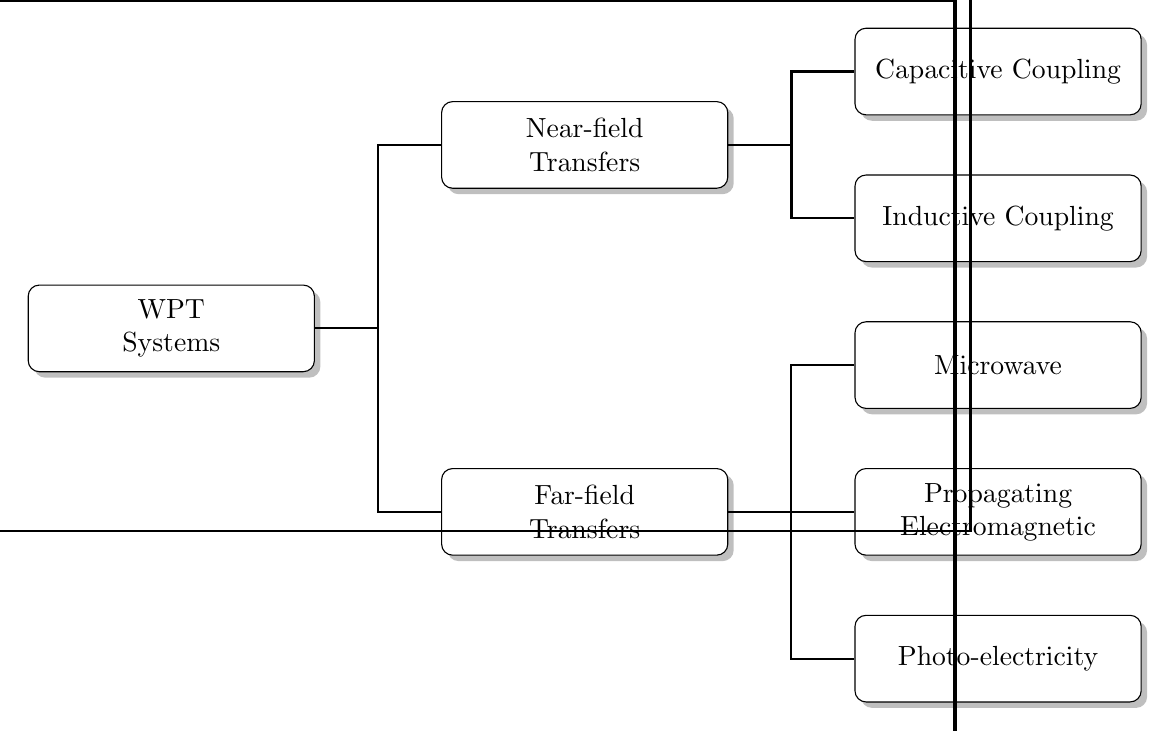
\begin{tikzpicture}[  grow'=right,
                      level distance = 5.25cm,
                      sibling distance = 0.75cm
                    ]

\tikzset{edge from parent/.style = {thick, draw, edge from parent fork right},
         every tree node/.style =
            {rectangle,rounded corners,drop shadow,draw,fill = white,minimum width = 2.8cm, minimum height = 1.1cm,text width = 3.4cm,align = center, text = black}}

\Tree 
    [. {WPT\\ Systems} 
        [.{Near-field\\ Transfers}
            [.{Capacitive Coupling} ]
            [.{Inductive Coupling} ]
        ]
        [.{Far-field\\ Transfers}
            [.{Microwave} ]
            [.{Propagating\\ Electromagnetic} ]
            [.{Photo-electricity} ]
        ] 
    ]

\end{tikzpicture}
\caption{Types of wireless power transfer inside the EM spectrum}
\label{fig:classification}
\end{figure}

%--------------

\section{Discussion}\label{sec:discussion}

% The inductive coupling is the only viable power transfer method which met all the requirements in terms of power and efficiency. It also accomplishes the first and one of the most important proposal in this work, to design a small wireless transfer system capable to be carried in a nano quadcopter.

% Discussion Radiative vs. Non-radiative
In radiative techniques $\vec{E}$ and $\vec{B}$ field strength decreases with distance from the source as $1/r^2$ for the radiated power intensity of electromagnetic radiation. However, near-field $\vec{E}$ and $\vec{B}$ strength decreases more rapidly with distance, being proportional to $1/r^3$. We could think this can be a bother when transferring power. And that is true, but this effect is mostly notable when transmitting over long-distance, which is not the priority of the project. This advantage of far-field over near-field techniques lies on the capability to focus electromagnetic radiation by reflection or refraction into beams. To achieve this narrow beams are necessary antennas much larger than the wavelength of the waves, corresponding to frequencies above 1 GHz, in the microwave range or above. Far-field techniques were rapidly refused because of the physical constraints of the transmitter antenna size, discussed on section \ref{subsec:geo}.

% Discussion between Non-radiative 
Seeing all the available technologies scope inside non-radiative techniques it is quite reasonable to guide towards Resonant Magnetic Induction. This power transfer is reminiscent of the usual magnetic induction; however, the usual non-resonant induction is very inefficient for midrange applications which compromise distances from one antenna diameter up to ten times the antenna diameter \cite{Karalis200834}. % 1e6 más eficiente
As opposed to directed electromagnetic radiation, such as lasers, it does not need an uninterrupted line of sight between the source and the device, as well as a sophisticated tracking mechanism when the device changes its position.

In addition, the fact that magnetic fields interact so weakly with biological organisms is also important for safety considerations \cite{TechTalk}. Capacitive coupling was rejected because of safety issues related to the necessity of a high source voltage. 

To summarize, Resonant Magnetic Induction was the unique WPT system which met mostly all requirements. It allows us to transfer power, nearly omni-directional, over midrange distances in a efficient way. Furthermore, this WPT system is irrespective of the geometry of the surrounding space, with low interference and losses into environmental objects. It also accomplishes the first and one of the most important proposal in this work; to design a small wireless transfer system capable to be carried in a nano-quadcopter.


\begin{table}[ht]
\begin{center}
\begin{tabular}{|l|c|c|c|c|}
% \hline
\rowcolor{black!60}
\hline
\color{white}WPT system                    & \color{white}Frequency   & \color{white}Directivity   & \color{white}Range   & \color{white}Efficiency    \\ \hline %\hline
\rowcolor{gray!54}
Capacitive Coupling           & Low Hz$\sim$MHz     & Weak         & Short       & High             \\ \hline
\rowcolor{white}
Inductive Coupling            & Low Hz$\sim$MHz     & Weak         &  Short      & High             \\ \hline
\rowcolor{gray!40}
Propagating Electromagnetic   & Medium MHz$\sim$GHz       & Medium         &  Medium      & Medium             \\ \hline
\rowcolor{white}
Microwave   & High GHz$\sim$THz       & Strong         &  Long      & Low             \\ \hline
\rowcolor{gray!40}
Photo-electricity   & High $>$THz       & Strong         &  Long      & Low             \\ \hline % Light waves

\end{tabular}
\caption{A comparison among the wireless power transfers}
\label{T:types}
\end{center}
\end{table}

\chapter{Modeling Magnetic Induction System}\label{C:modeling}

% , we opt for model C for being the most adequate in shape and for working in conjunction with the quadcopter. Model A has a radius too small for landing maneuvers. On the contrary, model B has a radius bigger than the quadcopter complicating the coil support. 




% \begin{table}[ht]
% \centering
% \begin{tabular}{|c|c|c|c|c|c|}

% \noalign{\global\arrayrulewidth1pt}
% \hline
% \textbf{Model name}  &   \textbf{Inductance} 	&   \textbf{Resistance} 	&   \textbf{Q factor} 	&   \textbf{Capacitor}  \\
% \hline
% \hline
% % \tablefootnote{The low inductance and resistance values of model A are due to weight restriction. Model A is a 23\% shorter than other models. By winding one turn involved to exceed mass constraint. Bigger diameters required more adhesive fixation.}

% Model A 	& 7.62$\mu$H 	& 0.489$\Omega$   & 	97 		& 31 nF     \\ \hline 
% Model B  	& 12.72$\mu$H 	& 0.619$\Omega$   & 	129 	& 31 nF 	\\ \hline
% Model C 	& 13.26$\mu$H 	& 0.651$\Omega$   & 	127 	& 31 nF 	\\ \hline

% \end{tabular}
% \caption{Theoretical coil calculations for a test frequency of 1 MHz}
% \label{T:theoretical}
% \end{table}

 




\chapter{Architecture and Design of the WPT System} \label{C:architecture}
Once the inductive coupling system has been studied in detail, it is time to outfit the selected coil model C on the drone. The selection of this model is argued in Chapter \ref{C:experimental}, after all the measures are performed. In this chapter, the required circuits to design the WPT system are discussed. In the first section, the nano-quadcopter used is introduced and all its main features are explained, as well as the necessity of designing brand new motor mounts in order to support the coil. 

In the second part of the chapter, the architecture of the transmitter and receiver circuits is explained, as well as its design. The main feature of the WPT system lies on energy conversion. Hence, both the transmitter and the receiver circuits need of power converters. As shown in Figure \ref{F:blockDiagram} the transmitter includes a ultra low DC-DC converter and a DC-AC converter. At the receiving side, the power converters include at least an AC-DC converter. Later, for the used application, a DC-DC converter will be introduced for the battery recharging circuit.

%%%
%%%
%%% SE ESCOGE LA BOBINA C !!! EXPLICAR QUE TODO EL CAPITULO SE TIENE EN CUENTA
%%%
%%%

\begin{figure}[htb]
\begin{center}
\vspace{+0.5em}
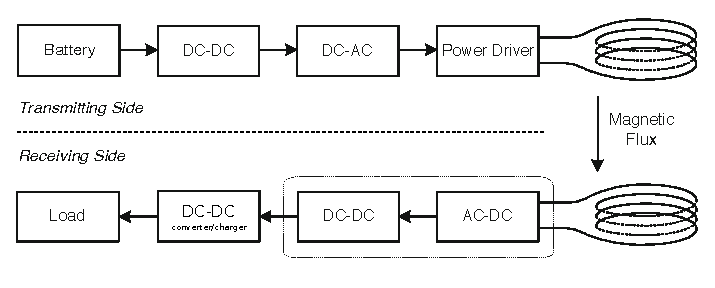
\includegraphics[width=0.9\textwidth]{./images/block2}
% \vspace{-1.5em}
\caption{Block diagram}
\label{F:blockDiagram}
\end{center}
\end{figure}


  \section{Quadcopter}
One of the initial objectives of the project is the WPT system outfitting on the nano-quadcopter. The inclusion of the quadcopter as an energy \textit{transporter} restricts both transmitter and receiver side, but mainly the transmitter because of the weight. The model used in this work is the created by \textit{Bitcraze}, its second nano-quadcopter version, named \textit{Crazyflie 2.0}. 

The assembly of this quadcopter can be divided into two parts. The first is composed by the battery, motors and headers attaching. In the second, the propellers are introduced and balanced. This last procedure is really important due the fact that well balanced propellers reduce vibrations in the copter and noise in the sensors improving the stability of the \textit{Crazyflie}.


\begin{figure}[H]
\centering
\begin{subfigmatrix}{2}
\vspace{1em} 
\hspace*{\fill}%
\subfigure[Crazyflie 2.0] 
  {\includegraphics[width=2.2in]{./images/crazyflie}}\hfill 
\subfigure[CrazyRadio USB dongle]
  {\includegraphics[width=2.0in]{./images/CrazyRadio}}
\hspace*{\fill}%
\end{subfigmatrix}
\caption{Transmitter circuit}
% \label{F:transmitter}
\end{figure}

Contrary to other drones, \textit{Crazyflie} allowed us the possibility to fly it indoor. It also has many interesting features listed in Table \ref{F:crazyflieFeatures} which made us to select it. Owing to the fact that \textit{Crazyflie} is an open source project it is possible to log, graph and set variables in real-time via the USB radio dongle.

\begin{figure}[htb]
\begin{center}
\begin{tabular}{|c|c|}

  \hline
  \multicolumn{2}{|c|}{\bf{Crazyflie 2.0 specification}} \\
  \hline
  \hline
  Size (WxHxD)  & 92x92x29 mm \\ \hline
  \multirow{2}{*}{Radio specs} 
   &  Low energy Bluetooth\\
   &  Radio amplifier 1 km range \\ \hline
  \multirow{3}{*}{Controllers} 
   &  STM32F405 MCU\\
   &  $\mu$USB connector \\
   &  USB OTG capability \\ \hline
  \multirow{3}{*}{IMU} 
   &  3 axis gyro \\
   &  3 axis accelerometer \\
   &  3 axis magnetometer \\
   &  Pressure sensor \\
  \hline

\end{tabular}
\caption{Crazyflie 2.0 features}
\label{F:crazyflieFeatures}
\end{center}
\end{figure}


    \subsection{Controlling the \textit{Crazyflie}}
As it is shown in Table \ref{F:crazyflieFeatures}, the \textit{Crazyflie} can be either controlled by a mobile device or a computer. Using a mobile device is the fastest way to control it, but its maneuverability is reduced compared to the computer option. Therefore, this last one is chosen.

The two needed requirements for flying the \textit{Crazyflie} using a computer are: a radio USB dongle (\textit{Crazyflie PA}) for communication and a standard gamepad for maneuvering. In addition, a virtualization program is required to run the \textit{Crazyflie} client. Few drivers are needed, as well as the last updated software in order to avoid any \textit{bug}. Both drivers and the needed code are uploaded on \textit{GitHub} repositories \cite{github}. 

\begin{figure}[H]
\centering
\includegraphics[width=0.65\textwidth]{./images/virtual}
\caption{Crazyflie's computer client}
\end{figure}


  \subsection{Motor Mount Design}

With the original design of the \textit{Crazyflie} nano-quadcopter is almost impossible to install it the used coil. As a consequence, in this case, the coil would not be subjected neither precisely, nor ``smartly''. The solution is to redesign the motor mounts of the \textit{Crazyflie} to accomplish a good coil support.

Using the CAD software \textit{SolidWorks}, it has been designed a motor mount with the same characteristics of the original mounts. The only difference is that the designed structure is made to place the coil under the \textit{Crazyflie}. 


This structure has the main characteristic of supporting lateral stresses, as the \textit{default} mounts, and also to prevent the fall of the coil, by using a kind of hook placed at the end of the mount arm. The complete design schematics are located in the Appendices. All this mentioned characteristics are showed in Figures \ref{F:MM} and \ref{F:MMC}. 

\begin{figure}[H]
\centering
\begin{subfigmatrix}{3} 
\subfigure[Plan and elevation views] 
  {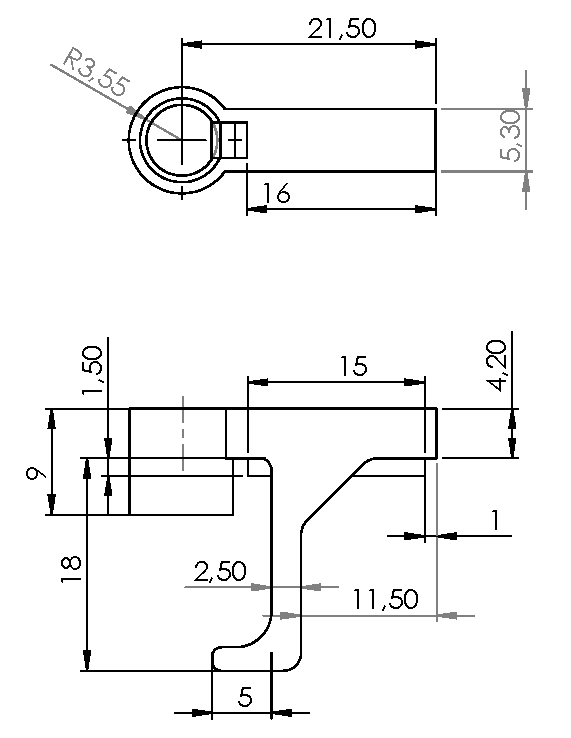
\includegraphics{./images/plantaAlzado}\label{F:MM}}
\subfigure[3D model] 
  {\includegraphics{./images/3dmount}\label{F:MMC}}
\subfigure[Real view image]
  {\includegraphics{./images/FullSizeRender}\label{F:finalMount}}
\end{subfigmatrix}
\caption{Motor mount process design}
\end{figure}

Once the motor mount is designed it can be printed with a 3D printer. The result is exhibited in Figure \ref{F:finalMount}.



  \section{Transmission System}

In a WPT system, the transmitter is intended for carrying power in order to satisfy the receiver demand. Its design is based on two premises; size and weight. Size is important in order to maintain the nano-quadcopter balanced owing to \textit{Crazyflie} is not designed to carry objects. The weight constraint is repeated several times during this project.

% Therefore, weight is the parameter which will define transmission subsystems.

    \subsection{Power Source}
After considering different options, such as using two isolated batteries for feeding the drone and the induction system separately, we decided to use the default battery of the nano-quadcopter, and so avoiding to increase the total weight. The battery \textit{Crazyflie} uses is of the type LiPo (Lithium-Polymer).
    
\begin{figure}[htb]
\begin{center}
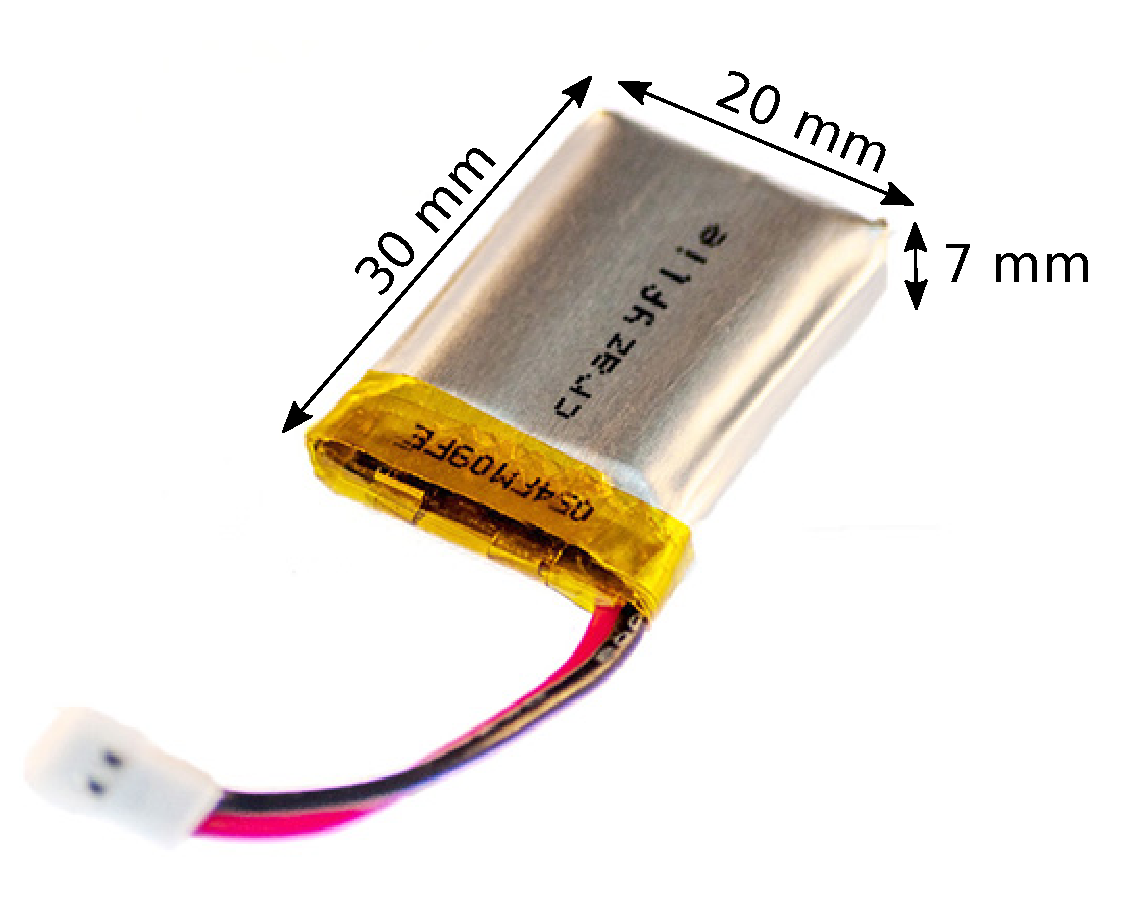
\includegraphics[width=0.4\textwidth]{./images/battery}
\caption{Crazyflie's battery size}
\label{F:battery}
\end{center}
\end{figure}

Althought LiPo is not the safest chemistry, these batteries are currently the most popular type for radiocontrol use. The reason is due to LiPo batteries has the best power to weight ratios and discharge currents. It also allows to use only a single cell.


\begin{table}[ht]
\begin{center}
\begin{tabular}{|c|c|c|c|}

\noalign{\global\arrayrulewidth1pt}
\hline
\textbf{Capacity}  &   \textbf{Nominal voltage}   &   \textbf{Discharge}    &   \textbf{Charge}\\
\hline
\hline
240 mAh   & 3.7 V   &   15C   &   2C  \\ \hline 

\end{tabular}
\caption{Battery's electrical specifications}
\label{T:batterySpecs}
\end{center}
\end{table}

The electrochemical batteries have the advantage over other energy storage devices, such as supercapacitors, that their main discharge curve is exponential, meaning that the energy stays high during most of the charge and then drops rapidly as the charge depletes \cite{batteryDischarge}. The \textit{Crazyflie} battery discharge rate or C-rate is of 15C which means 15-times the rated capacity.

As it is stated in \cite{crazyflie}, the maximum flight time with LiPo battery is up to 7 minutes. Theoretically with motors at full power and consuming 3600 mA, the flight is being reduced to 4 minutes. Regrettably, this time will be even reduced by the inclusion of the induction system. 

The end-of-discharge voltage for most LiPo is 3.0 V/cell. At this level, roughly 95 percent of the energy is spent and the voltage would drop rapidly if the discharge were to continue \cite{batteryDischarge}. To protect the battery from over-discharging, which is very sensitive to, the quadcopter comes with a PCM (Protection Circuit Module) that prevents operation beyond a specified end-of-discharge voltage. 










\subsection{Voltage Regulator}
The voltage regulator was the last system implementation. Owing to the necessity of having 12 V, explained in Chapter \ref{C:experimental}, on the transistor collector, a switching voltage regulator is the most appropriate solution. Linear regulators can only step down the input voltage and the possibility of adding a second battery was rejected because of weight. 

Switching regulators are highly efficient and able to boost, buck and invert voltages with ease, but they also have weaknesses. One of them is that they are complex chips and, consequently, it can take a lot of design effort to get a new product working properly. In addition, the level of integration of contemporary switching regulators does not come cheaply and increases the chip size \cite{regulators}.

To solve these issues the \textit{Webench} application is used. This design tool developed by \textit{Texas Instruments} allows to design the voltage regulator that better adjusts to our input and output power requirements. 

\begin{table}[htb]
\begin{center}
\begin{tabular}{|c|c|c|}

\noalign{\global\arrayrulewidth1pt}
\hline
\textbf{Input Voltage}  &   \textbf{Output Voltage}   &   \bf{Output Current}\\
\hline
\hline
3 - 3.7 V       & 12 V   &   0.5 A  \\ \hline 

\end{tabular}
\caption{Regulator requirements}
\label{T:regulator}
\end{center}
\end{table}

\begin{figure}[H]
  \begin{center}
    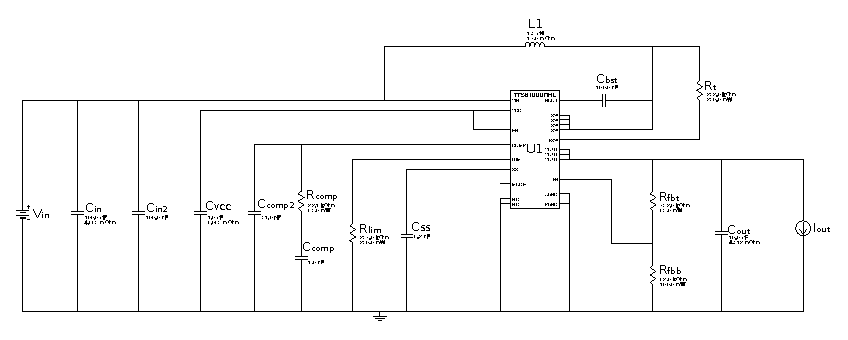
\includegraphics[width=1.05\textwidth]{./images/TPS61088}
  \caption{TPS61088 design circuit}
  \end{center}
\end{figure}

It must be said that the regulator is designed to provide a maximum output current of 500 mA, which is the maximum input current of the power driver, discussed later.

The requirements above lead us to different switching regulators. By looking at size and efficiency, the TPS 61088 was the one with best efficiency per unit of area. The circuit schematic is given in Appendix \ref{Appendix: DC-DC}.

Although an ideal switcher has a $100\%$ efficiency, the actual efficiency is about $92\%$ (Appendix \ref{Appendix: DC-DC}) and it depends on the output current and the input voltage. The power \textit{lost} is really low and it is dissipated following,

\begin{equation}
P_{dis} = \left(\frac{1}{\eta}-1\right)\cdot{P{out}}
\end{equation}


The input current that the regulator is drawing to the battery can be calculated using Equation \ref{eq:regulator}, and it defines the global circuit consumption. 

\begin{equation}\label{eq:regulator}
I_{in} = \left({I_{out}}\cdot\frac{V_{out}}{V_{in}}\right)/{\eta}
\end{equation}

Before computing $I_{in}$, it will be necessary to figure out which is the output current and which relies on the power driver. 









    \subsection{Oscillator} 
A Quartz Crystal Oscillator (XO) is used to generate the necessary periodic signal which generates the alternating current in the \textit{Tx} coil. It is selected for its good performance, a low power consumption, and a simple electronic circuit. This type of oscillator not only provides an extraordinary frequency stability, but it also provides a constant frequency output under varying load conditions, which is an important aspect to consider.

\begin{figure}[H]
\begin{center}
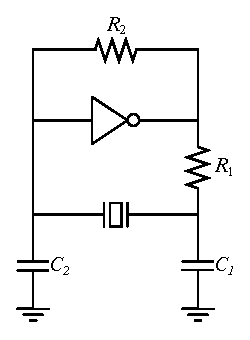
\includegraphics[width=0.3\textwidth]{./images/oscilador}
\caption{Oscillator schematic}
\label{F:oscillator}
\end{center}
\end{figure}

The functioning of the quartz crystal oscillator is based on piezoelectric effect. Piezoelectricity is the primary property of a crystal which makes it usable as resonator. Piezoelectricity is a reversible property of a crystal by which an electrical charge produces a mechanical force by changing the shape of the crystal and vice versa, a mechanical force applied to the crystal produces an electrical charge \cite{quartzCrystal}. 

As it is discussed at the end of the previous chapter, each coil model has its own resonant frequency, and therefore a unique oscillator circuit. For the selected coil model, the resonant frequency is 0.95 MHz. 

The characteristic frequency of the crystal, or rate of vibration, is determined by the cut, size, and shape of the quartz crystal. Therefore, to achieve the desired frequency of 0.95 MHz a special crystal is needed. Hence, taking advantage on the wide Q factor of coils, an standard crystal frequency of 1 MHz is selected. 

\begin{table}[htb]
\begin{center}
\begin{tabular}{|c|c|}

\noalign{\global\arrayrulewidth1pt}
\hline
\textbf{Parameter}  &   \textbf{Value}\\
\hline
\hline
Frequency       & 1 MHz                  \\ \hline 
$R_1$           & 9.1 M$\Omega$          \\ \hline 
$R_2$           & 910 $\Omega$           \\ \hline 
$C_1$           & 47 pF                \\ \hline
$C_2$           & 47 pF                \\ \hline  
Consumption     & 8.4 mA                 \\ \hline

\end{tabular}
\caption{XO parameters}
\label{T:XOparameters}
\end{center}
\end{table}


In figure above, it is represented the Pierce oscillator circuit. This parallel oscillator is a derivative of the Colpitts oscillator. The circuit is implemented using a minimum of components: a single CMOS inverter gate, two resistors, two capacitors and the quartz crystal.

For high speed CMOS logic families, typically \cite{oscilador}:
\begin{itemize}[noitemsep] % To be more compact --> \begin{itemize}[noitemsep,nolistsep]
  \item $R_1$ is between 8.2 M$\Omega$ and 10 M$\Omega$
  \item $R_2$ is between 470 $\Omega$ and 2220 $\Omega$
  \item $C_1$ and $C_2$ are of the order of 62 pF 
\end{itemize}









    \subsection{Power Driver}

The output power delivered from the oscillator is not enough to feed the inductor directly. Thus, a Darlington transistor has been placed after the oscillator to elevate the magnetizing current through the primary coil. This increase in the input power will allow the system to transfer power up to larger distances.

The ULN2803A driver is a high-voltage, high-current Darlington transistor array. The device consists of eight NPN Darlington pairs that feature high-voltage outputs with common-cathode clamp diodes for switching inductive loads. Figure \ref{F:transitor} shows a simplified scheme of the power driver. The complete scheme is attached at Appendix \ref{Appendix: powerDriver}.

\begin{figure}[h]
  \begin{center} 
  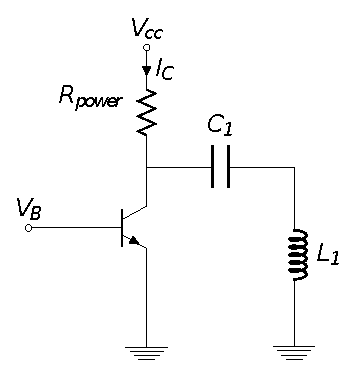
\includegraphics[width=0.4\textwidth]{./images/transistor}
    \caption{Simplified transistor diagram}
    \label{F:transitor}
  \end{center}
\end{figure}

From Figure \ref{F:transitor}, it can be observed that the transistor is working such a switch and driven by the square signal of 0-12 V coming from the oscillator. When an input (pins 1 to 8) is driven ``HIGH'' the corresponding output will switch ``LOW'' sinking current. Likewise, when the input is driven ``LOW'' the corresponding output switches to a high impedance state. This high impedance ``OFF'' state blocks load current and reduces leakage current through the device improving efficiency.

\begin{table}[htb]
\begin{center}
\begin{tabular}{|c|c|}

\noalign{\global\arrayrulewidth1pt}
\hline
\textbf{Parameter}  &   \textbf{Value}\\
\hline
\hline
$V_{CC}$            & 12 V            \\ \hline 
$V_{CE(SAT)}$       & 1.3 V           \\ \hline 
$I_{CC(MAX)}$       & 500 mA          \\ \hline 
$R_{power}$         & 33 $\Omega $      \\ \hline
\end{tabular}
\caption{Electrical characteristics}
\label{T:transistor}
\end{center}
\end{table}


Pin 8 (GND), is connected to the loads ground or 0 volts, while pin 10 ($V_{CC}$) connects to the loads supply. Then any load needs to be connected between +$V_{CC}$ and an output pin, pins 11 to 18. For inductive loads such as coils, pin 10 should always be connected to $V_{CC}$.

The ULN2803A Darlington driver is capable of switching 500 mA per channel. In our case the collector-current $I_{CC}$ is determined using the next expression,

\begin{equation}
I_{CC} = \frac{V_{CC}-V_{CE(SAT)}}{R_{power}}=324\:\textnormal{mA}
\end{equation}

where $R_{power}$ is achieved by combining three resistors in parallel. Each resistor has a resistance value of 100 $\Omega$ and tolerates powers around 1W without any problems. Once the collector current is calculated, it is possible to calculate the total power demanded from the battery. Substituting $I_{CC}$ in equation \ref{eq:regulator} an input current of 1.05 A is obtained. Therefore, the total theoretical power consumed by the transmitter is:

\begin{equation}
P_{in} = V_{in}\cdot{I_{in}}=3.88\:\textnormal{W}
\end{equation} 

It must be also considered the maximum switching frequency of the ULN2803A. Table \ref{T:transistor2} exhibits the propagation delay-times. The most restrictive is the change from ``LOW'' to ``HIGH'' state which takes 130 ns. The delay time delimits a maximum operating frequency of 7.69 MHz. Lowering the operating frequency from this value ensures a better Darlington efficiency.

\begin{table}[htb]
\begin{center}
\begin{tabular}{|c|c|}

\noalign{\global\arrayrulewidth1pt}
\hline
\textbf{Propagation delay time}  &   \textbf{Value}\\
\hline
\hline
 High-Low       & 20 ns           \\ \hline 
 Low-High       & 130 ns          \\ \hline 
\end{tabular}
\caption{Switching characteristics}
\label{T:transistor2}
\end{center}
\end{table}


  \subsection{Transmitter Circuit Assembly}
A printed circuit board (PCB) is needed for physically supporting and wiring the transmitter circuits (regulator, oscillator and power driver). Working with SMD technology makes possible to reduce mostly all the components size. Its round shape is owing to the fact that weight must be distributed as close as possible to the center of gravity. The circular shape also allows to maximize the board space, as well as, not to disturb the coil placement.


\begin{figure}[H]
\centering
\begin{subfigmatrix}{2} 
\hspace*{\fill}
\subfigure[Front view] 
  {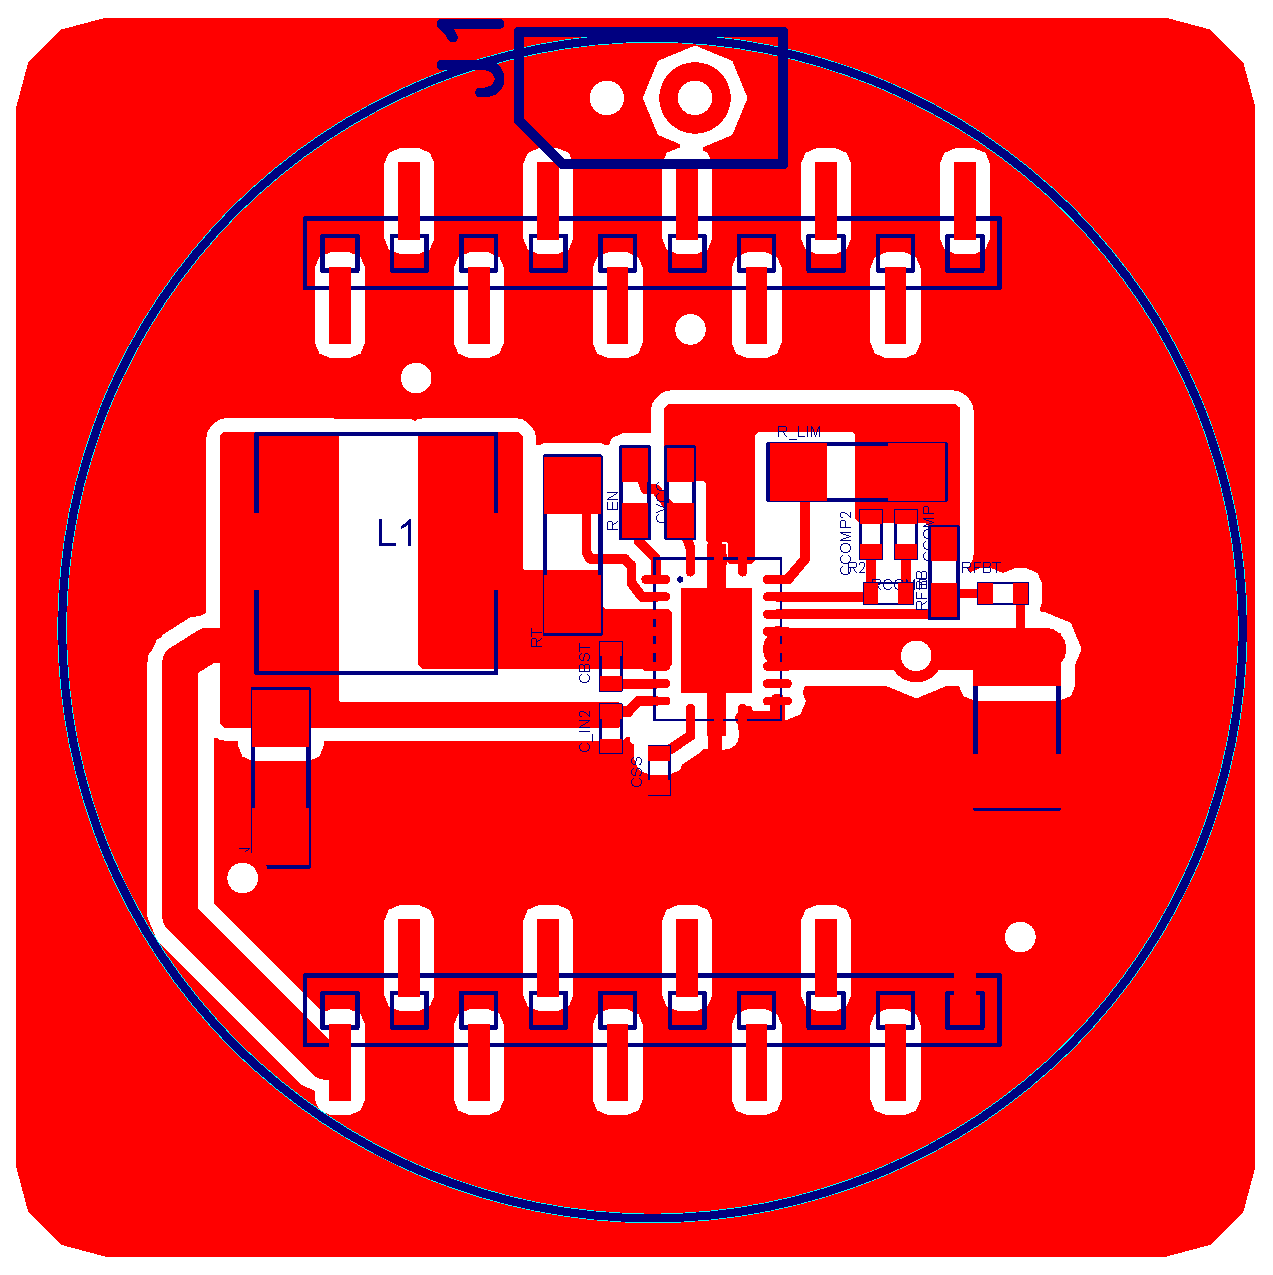
\includegraphics[width=2.0in]{./images/francis1}}\hfill
\subfigure[Back view]
  {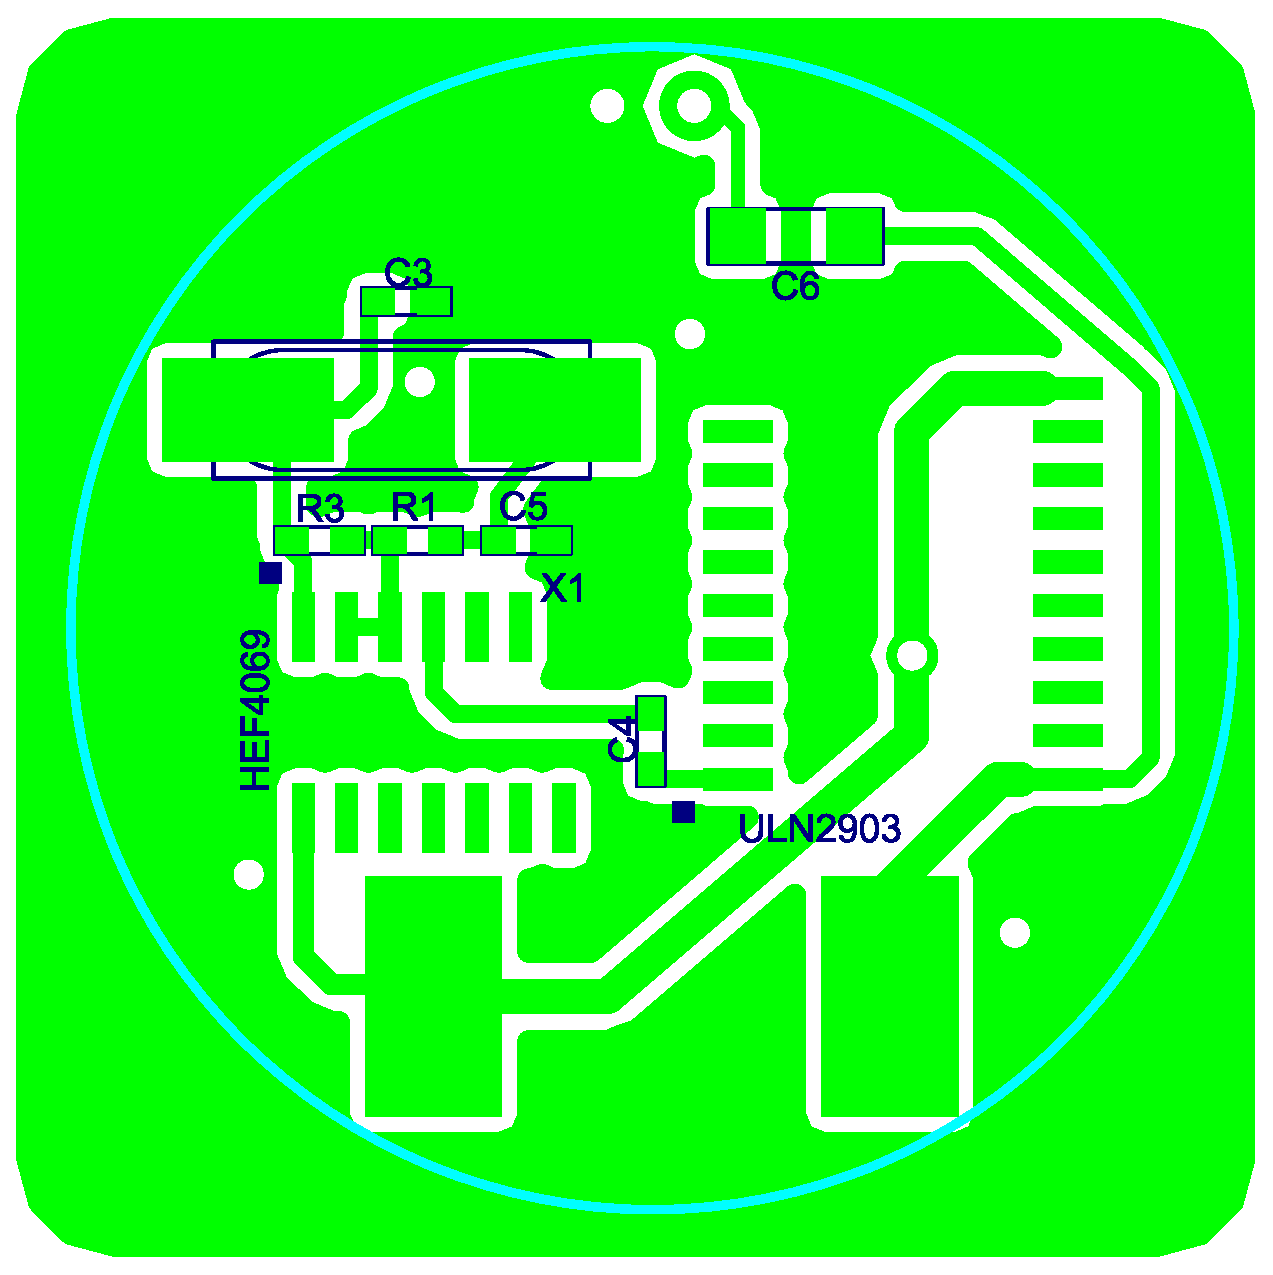
\includegraphics[width=2.0in]{./images/francis2}}
\hspace*{\fill}
\end{subfigmatrix}
\caption{Transmitter SMD design}
\end{figure}

Figure \ref{F:transmitter} exhibits the final transmitter board which is divided in two parts. The top side \ref{F:TX1} is composed by the power driver and the oscillator. It has the input coil pins to attach the primary inductor. The bottom side, invisible when the transmitter is connected to the \textit{Crazyflie}, is formed by the voltage regulator and the adapted pins. Those pins permit to connect directly the board to the quadcopter. The board height is small enough to avoid to graze the floor.


\begin{figure}[H]
\centering
\begin{subfigmatrix}{3}
\vspace{1em} 
\hspace*{\fill}%
\subfigure[Front view] 
  {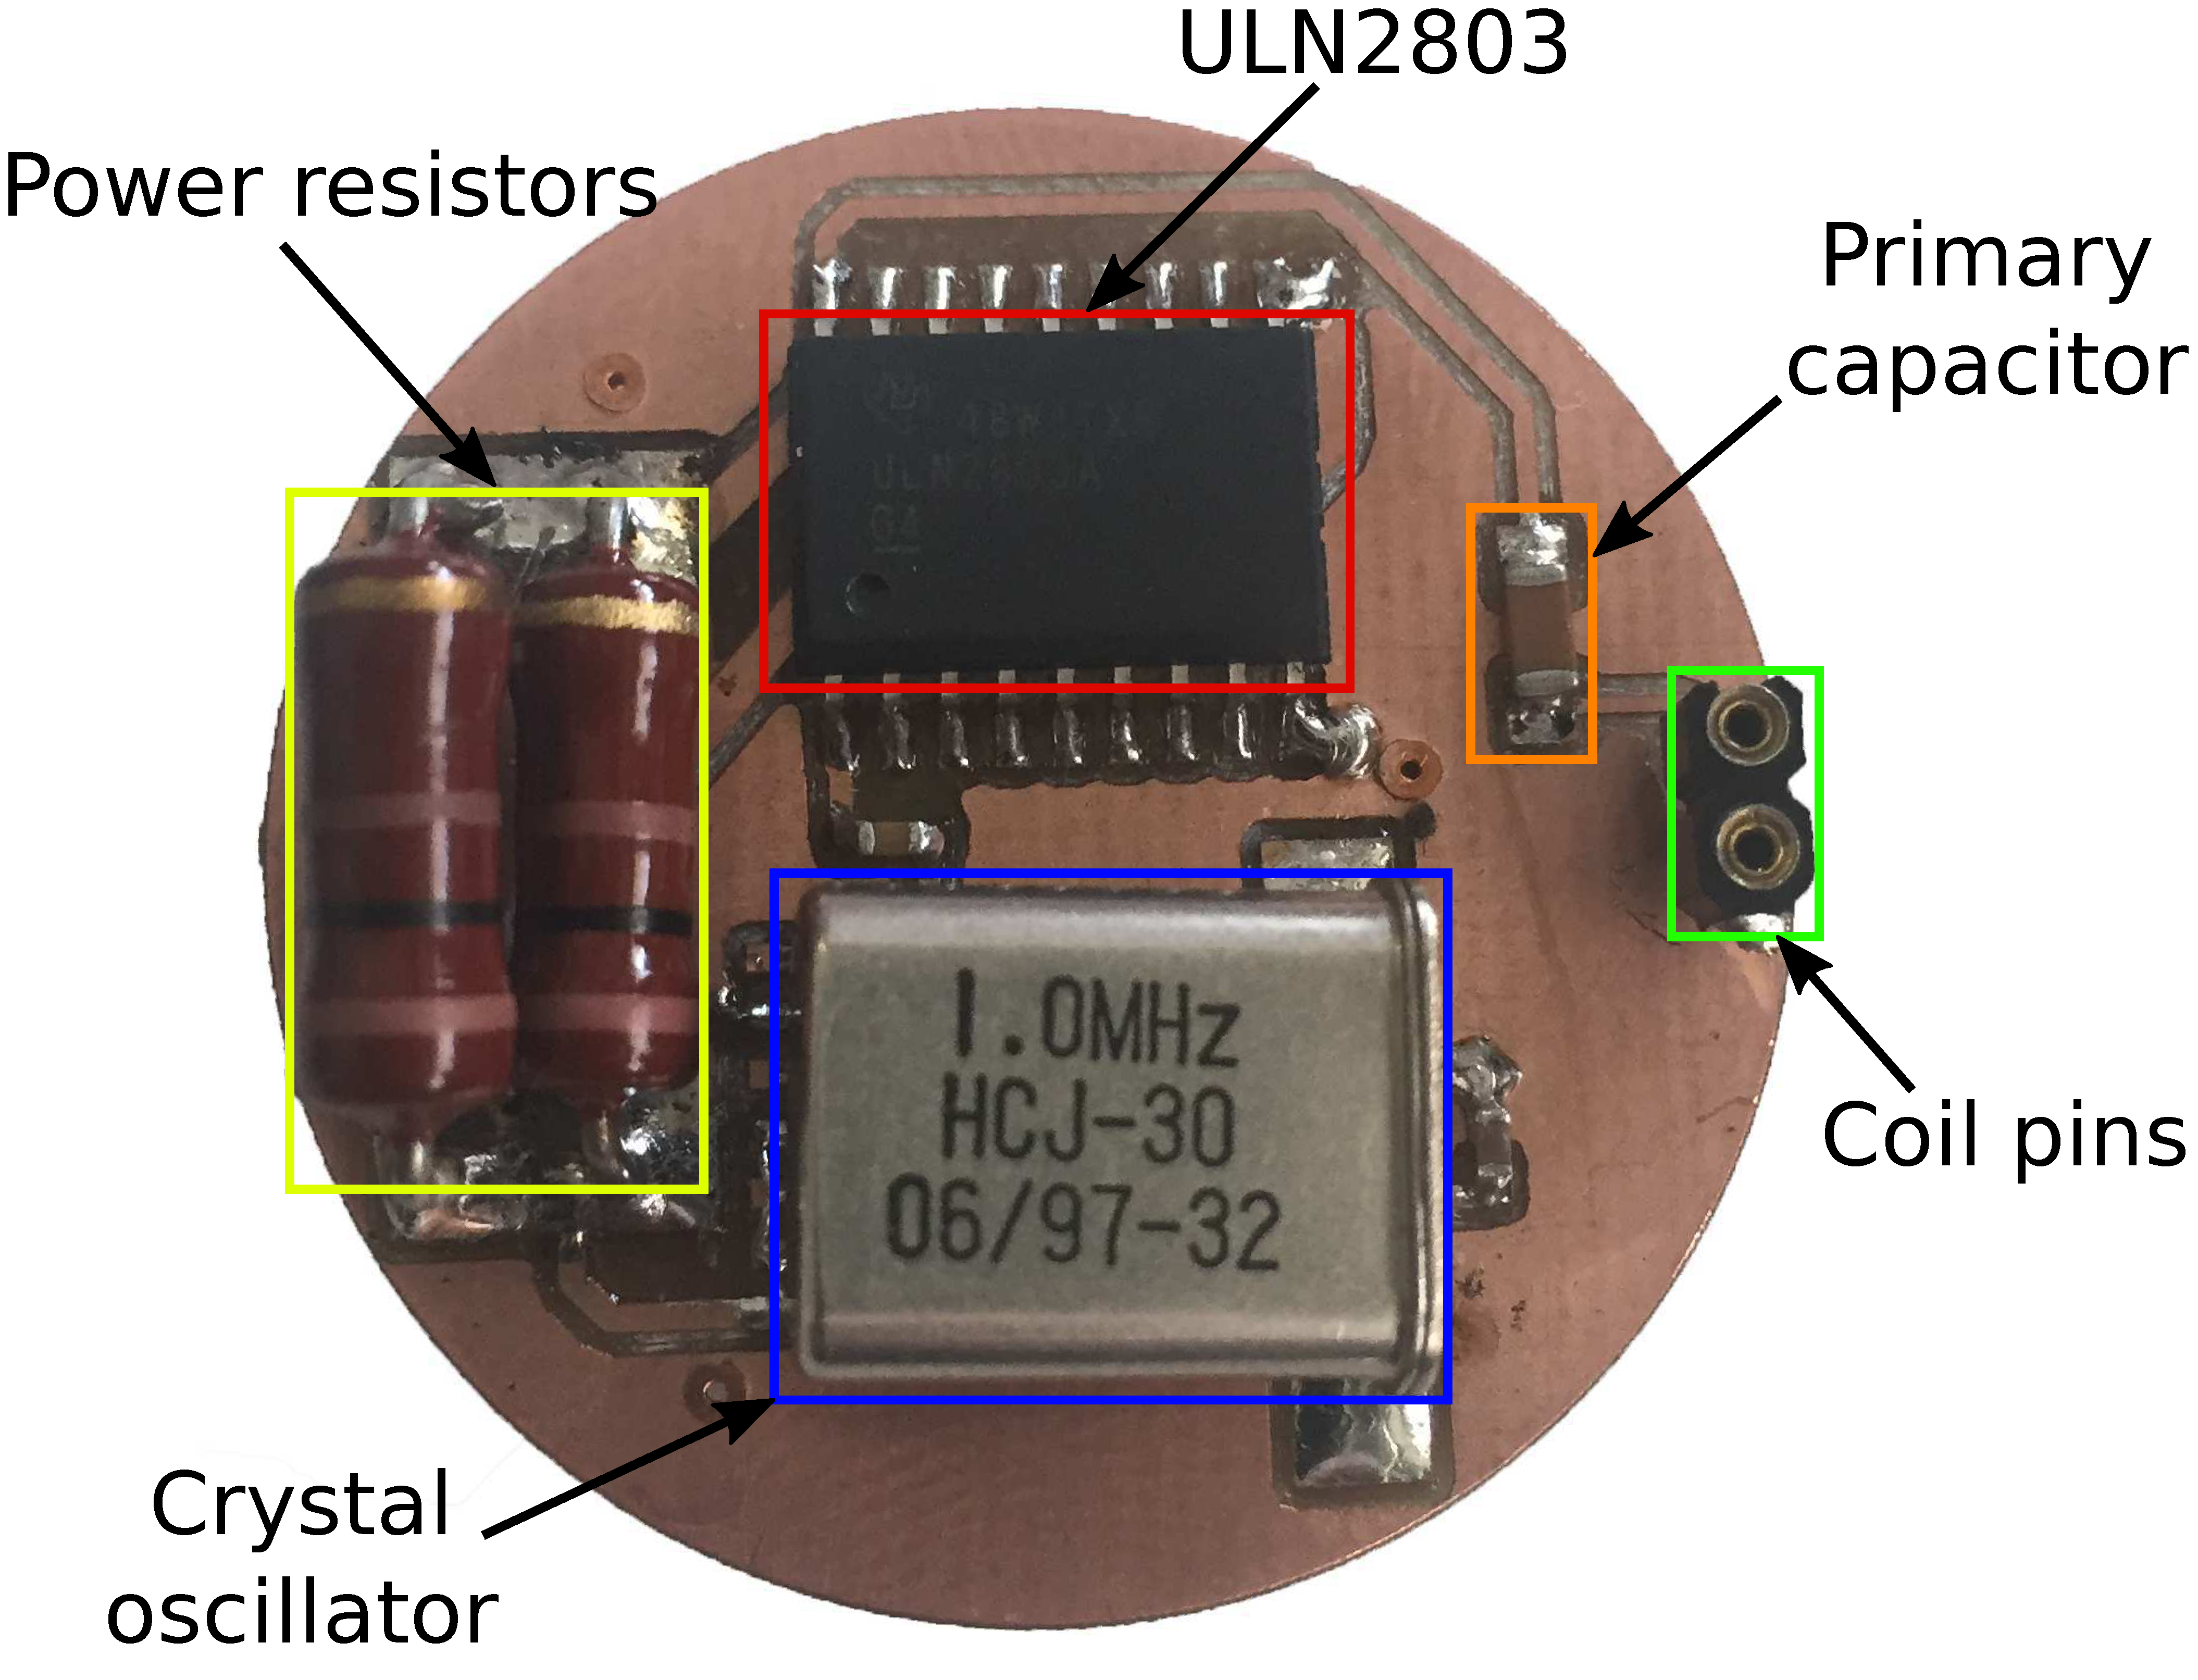
\includegraphics[width=2.0in]{./images/Transmitter_1X}\label{F:TX1}}\hfill
\subfigure[Side view] 
  {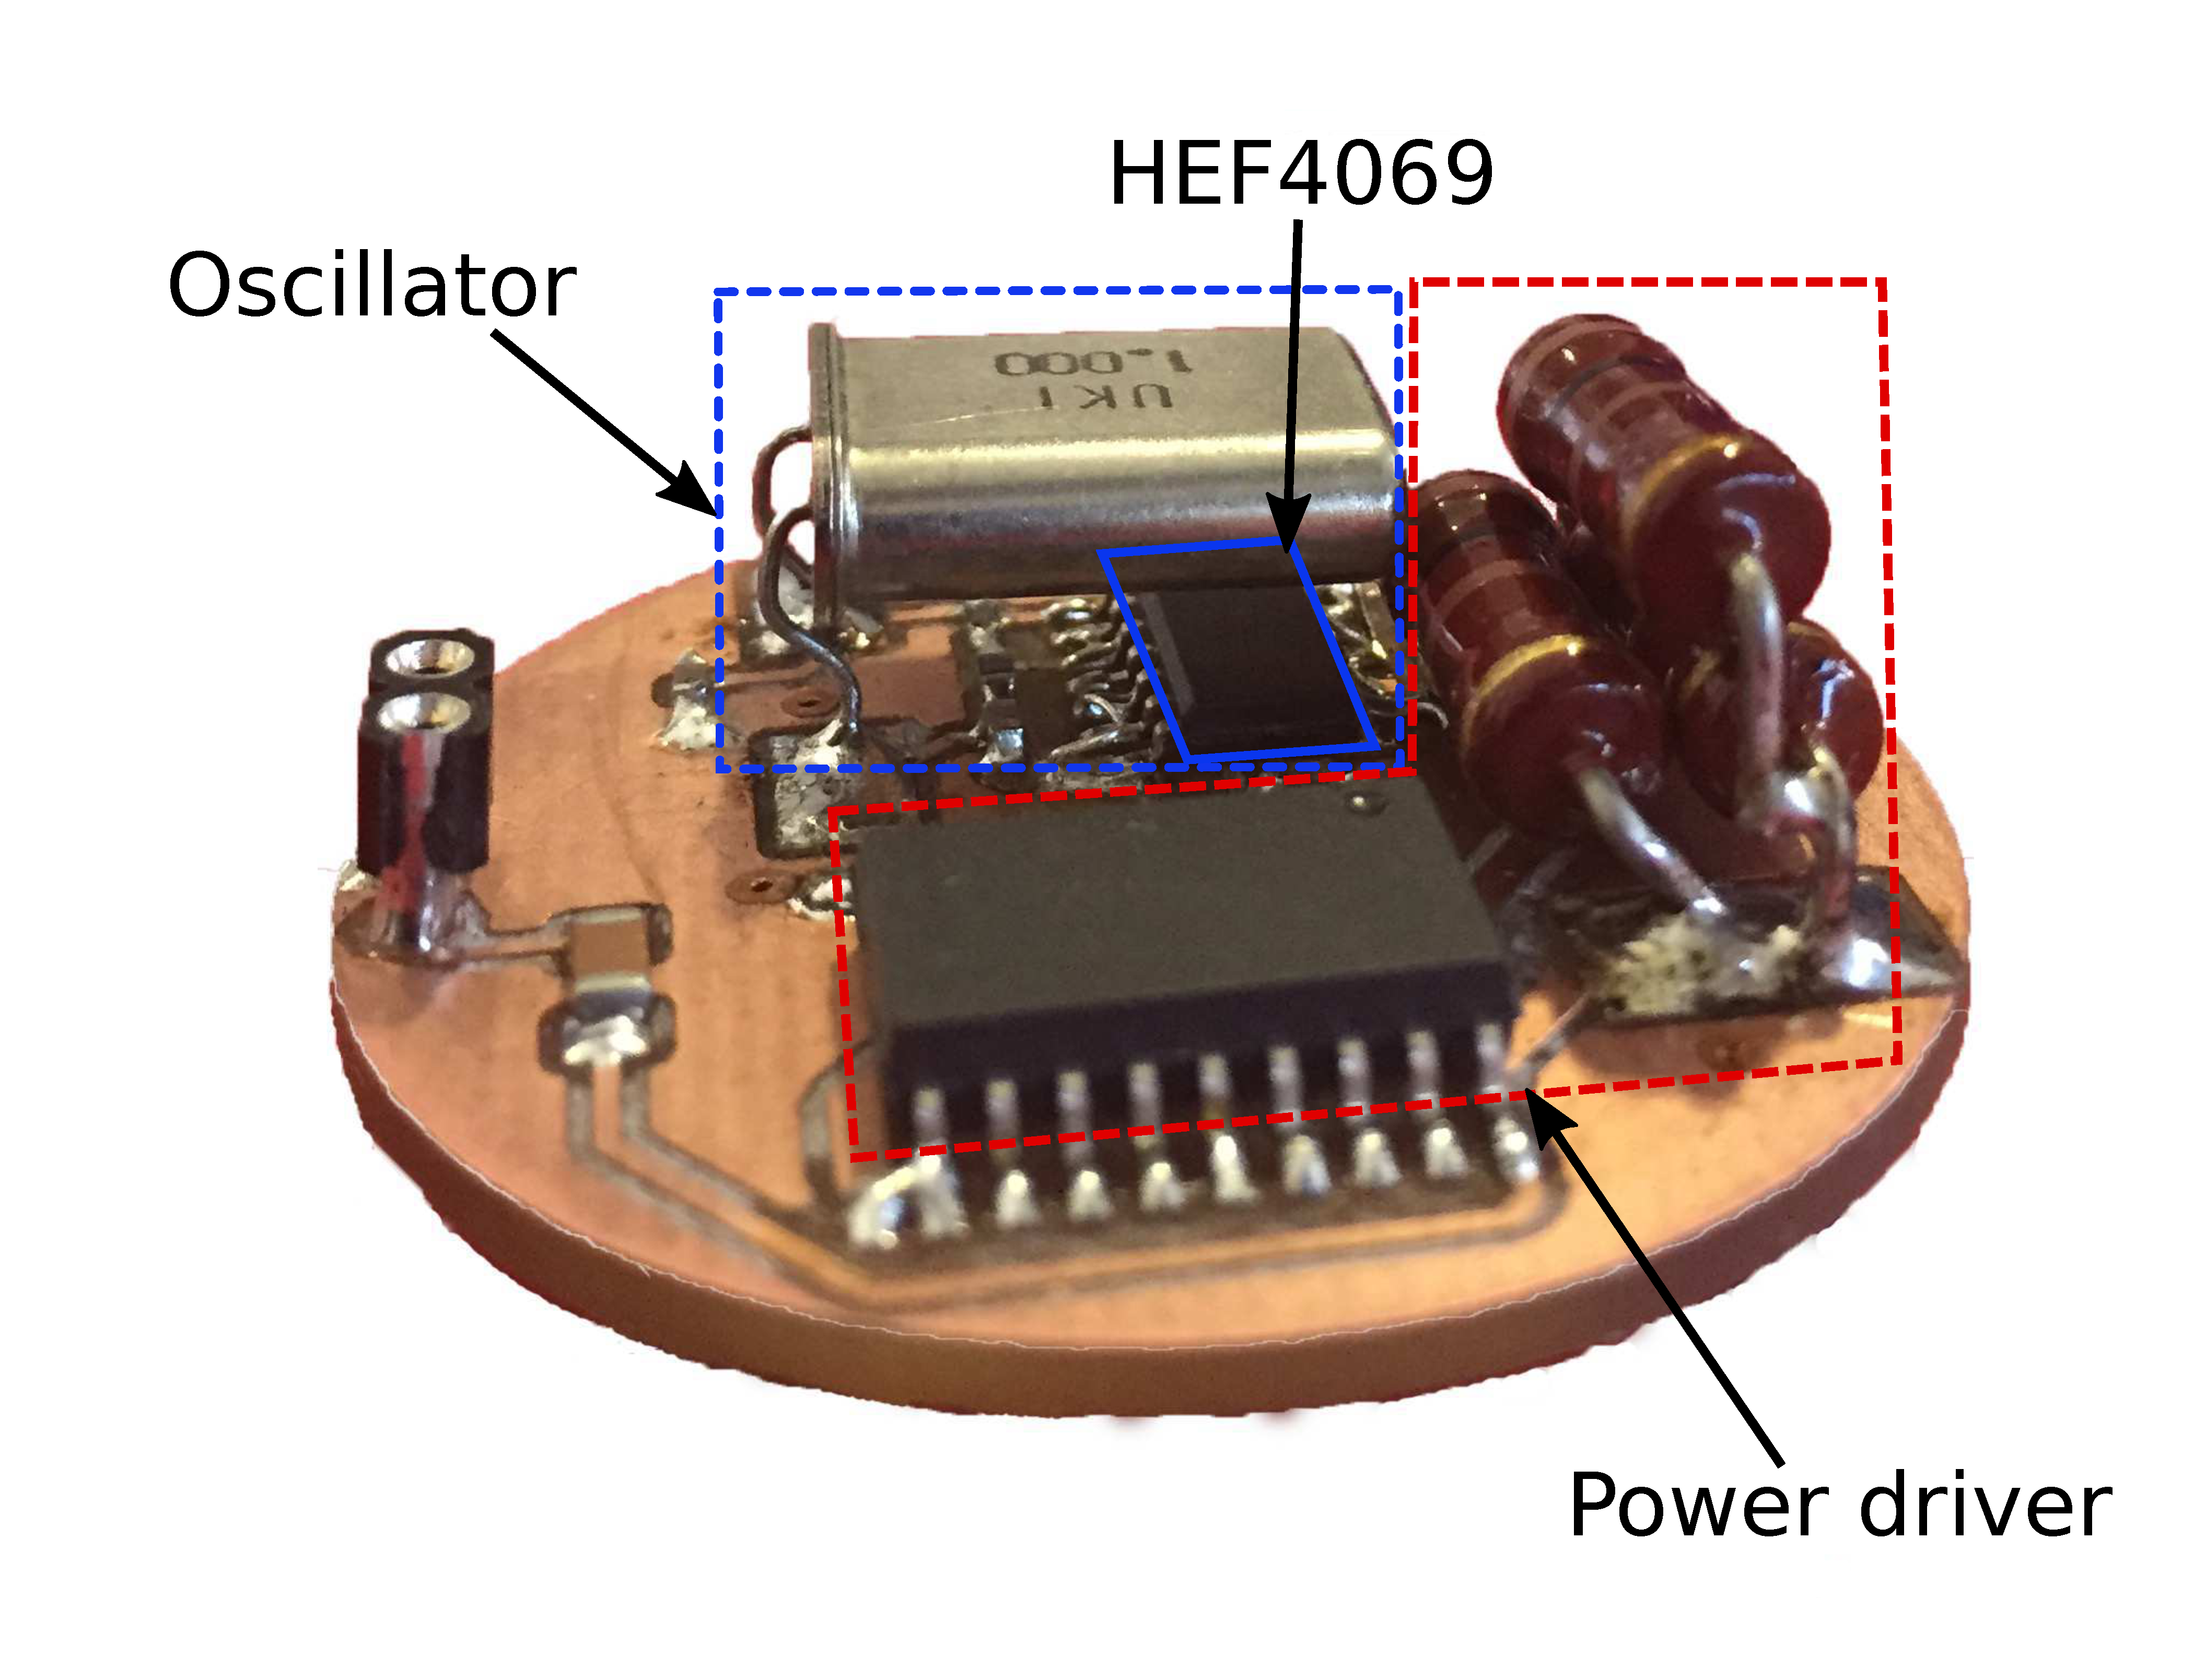
\includegraphics[width=2.0in]{./images/Transmitter_3}\label{F:TX3}}\hfill  
\subfigure[Back view]
  {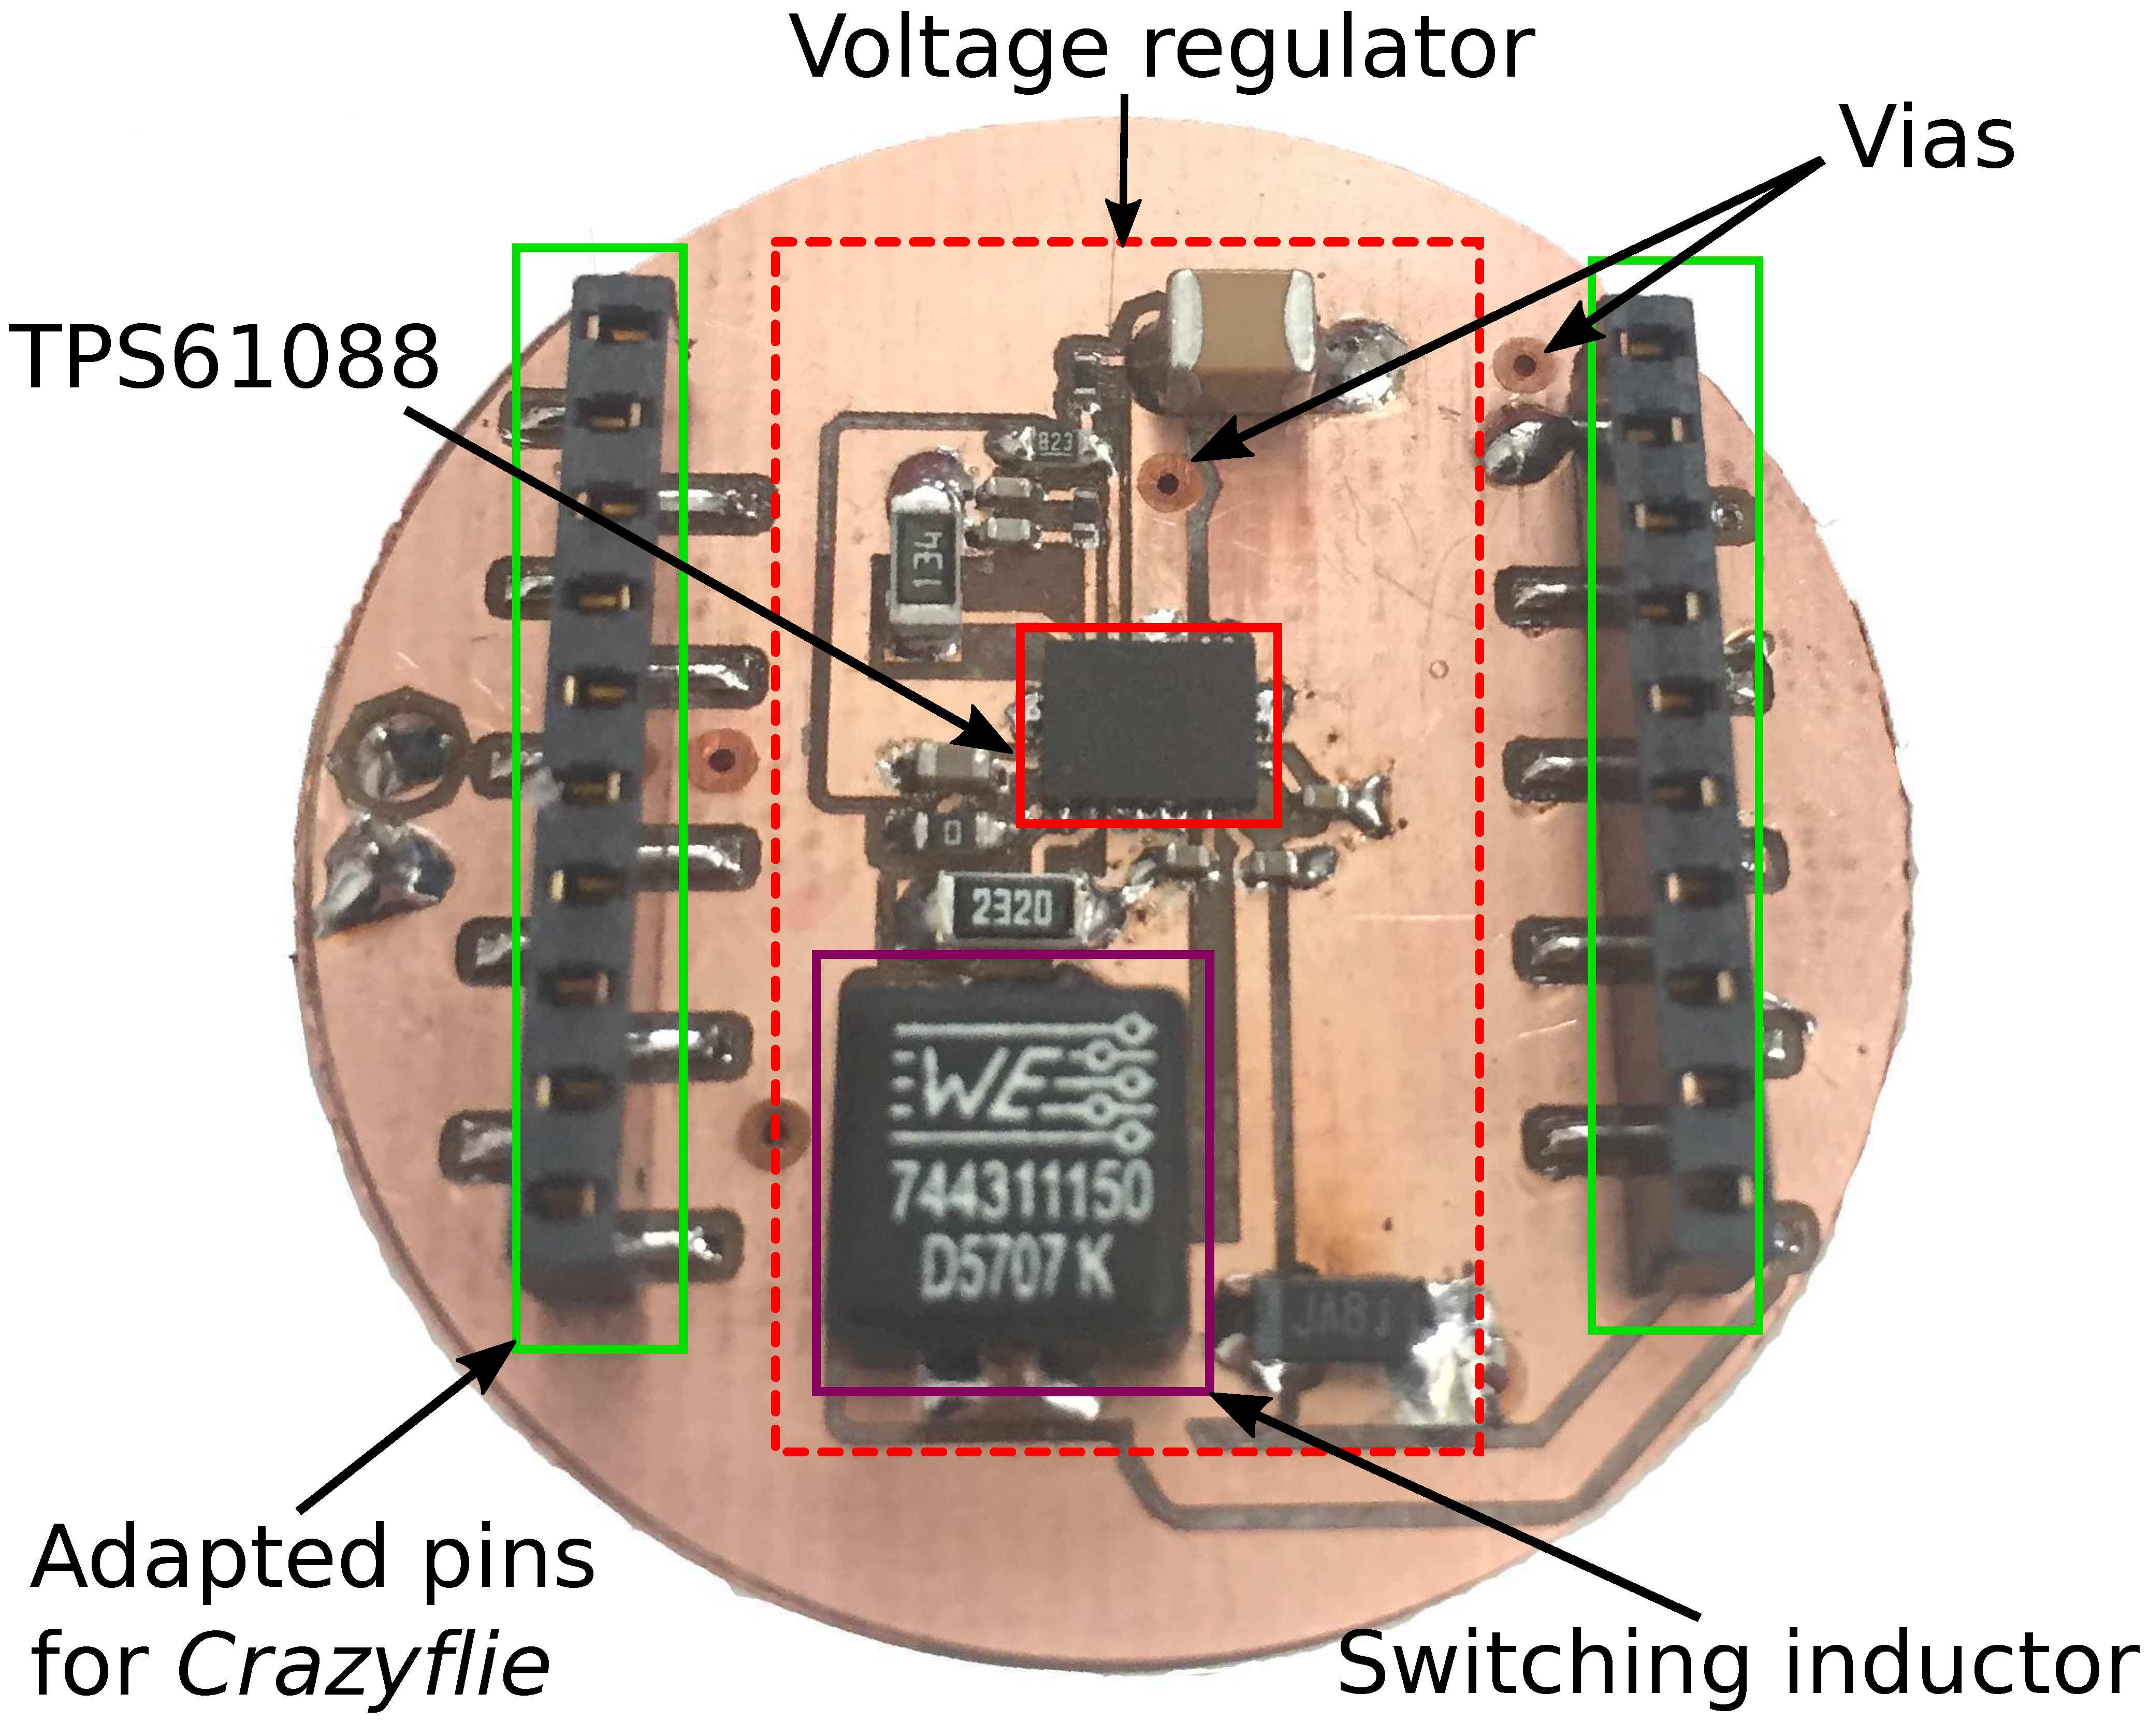
\includegraphics[width=1.9in]{./images/Transmitter_2Y}\label{F:TX2}}
\hspace*{\fill}%
\end{subfigmatrix}
\caption{Transmitter circuit}
\label{F:transmitter}
\end{figure}

Eventually, the total mass is computed using a precision scale. Table \ref{T:massConstraint} shows the mass of each section of the quadcopter. The experimental take-off mass depending on the motors thrust is shown in Figure \ref{F:thrust}. 

\begin{table}[htb]
\begin{center}
\begin{tabular}{|c|c|}

\noalign{\global\arrayrulewidth1pt}
\hline
\textbf{Element}  &   \textbf{Weight}\\
\hline
\hline
Battery             & 7.1 g     \\ \hline 
\textit{Tx} Coil    & 13.5 g    \\ \hline
\textit{Tx} Circuit & 8.5 g        \\ \hline
Crazyflie           & 8.3 g        \\ \hline
DC motors           & 4 x 2.8 g    \\ \hline
Motor mounts        & 4 x 0.8 g       \\ \hline
\hline
\textit{TOTAL}        & 51.8 g       \\ \hline

\end{tabular}
\caption{Mass constraint at transmitter side}
\label{T:massConstraint}
\end{center}
\end{table}


\begin{figure}[H]
  \begin{center} 
  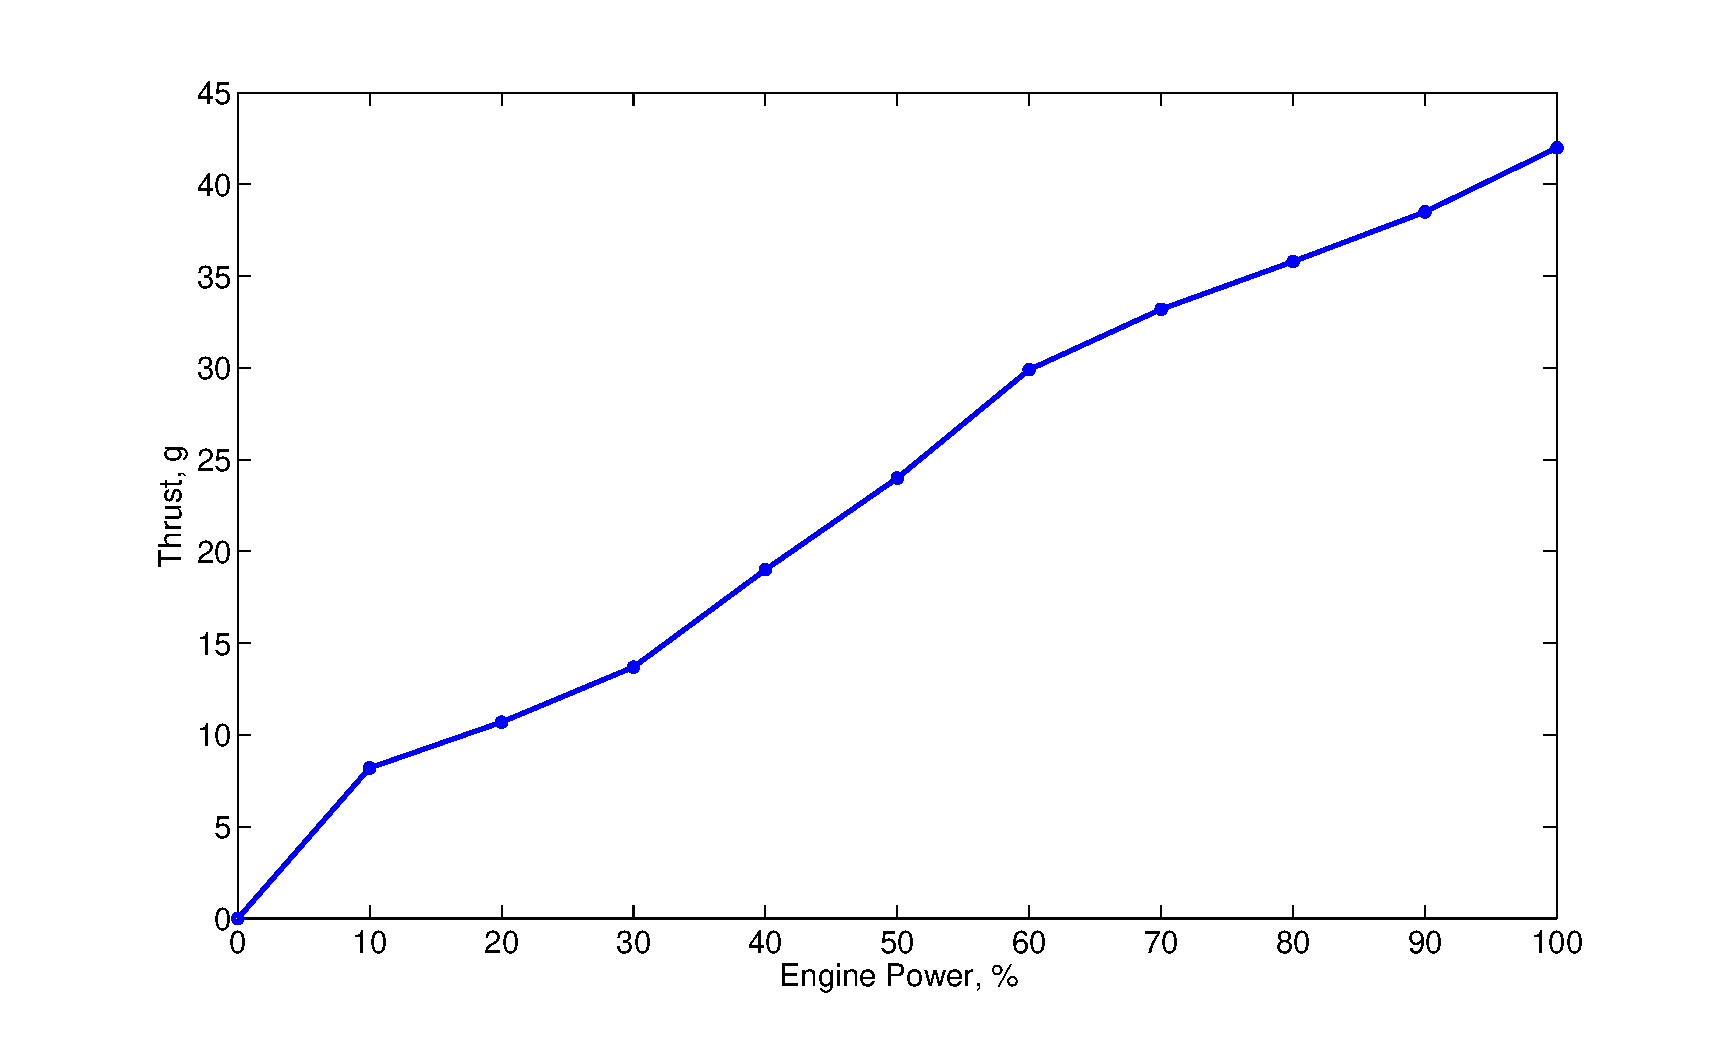
\includegraphics[width=0.9\textwidth]{./images/thrust}
    \caption{Thrust depending on the power level of the motors}
    \label{F:thrust}
  \end{center}
\end{figure}

\section{Receiver system}

The receiver side for a WPT system has the aim to rectify the transferred AC signal and, once it is in DC, to set it up to the desirable voltage levels. Depending on the application these two characteristic can be done in one stage. In the following sections the used circuits are explained in detail to accomplish a good signal rectification and conditioning. The chosen application for this project is presented is Section \ref{subsec:app}.

\subsection{Voltage Doubler}

To rectify the signal is selected a common used circuit for energy harvesting applications, the voltage doubler. This circuit is the perfect option for an energy harvesting. Owing to the low RF voltage levels, the doubler can rectify and condition at the same time. Voltage doubler circuits can be viewed as single stage or of a higher order multiplier; cascading identical stages together it is achieved a greater voltage multiplication. In Figure \ref{F:voltageDoubler} is shown a single stage for voltage doubler. 

\begin{figure}[ht!]
\begin{center}
\begin{circuitikz}
\ctikzset{v/.append style={/tikz/american voltages}}
\ctikzset{bipoles/resistor/height=0.25}
\ctikzset{bipoles/resistor/width=0.5}
\draw (0,2)
to[C=$C_1$] (2,2);
\draw (0,0)
to[short] (2,0)
to[D*] (2,2);
\draw (2,2)
to[D*] (4,2)
to[C=$C_2$] (4,0)
to[short] (2,0);
\draw (4,2)
to[short] (6,2);
\draw (4,0)
to[short] (6,0);
\node [ocirc] at (0,2) {$\qquad$};
\node [ocirc] at (0,0) {$\qquad$};
\node [ocirc] at (6,2) {$\qquad$};
\node [ocirc] at (6,0) {$\qquad$};
\node at (0,1) {$V_{in}$};
\node at (6,1) {$V_{out}$};
\node at (3,2.78) {$D_2$};
\node at (1.3,1) {$D_1$};
\end{circuitikz}
\caption{SIngle voltage doubler stage}
\label{F:voltageDoubler}
\end{center}
\end{figure}

An understanding of this circuit can be gained by interpreting firstly what occurs when the down swing of the AC current flows through the circuit. The diode $D_2$ blocks the current flow through $C_2$, but not the flow that goes across $C_1$. This current flow charges $C_1$ up to the same level of the AC voltage amplitude. Once the up swing of the AC voltage is reached, the voltage of both AC source and $C_1$ drop across $C_2$, charging it approximately twice the peak voltage of the AC signal \cite{doubler}.

As it is said in the first paragraph the voltage doubler is used in many energy harvesting applications, where the frequency goes from MHz to GHz. Thus, not all diodes are able to commute at these frequencies. The operating frequency of the inductive system of this project is set of 1 MHz and the selected diodes for assembling the voltage doubler are the HSMS-2850 Schottky diodes (SOT-23 Package) from \textit{Avago Technologies}:

\begin{figure}[htb]
\begin{center}

\includegraphics[width=0.2\textwidth]{./images/schottky}
\caption{SOT-23 Package for HSMS-2850 Schottky diode}
\end{center}
\end{figure}
The impedance of the HSMS-2850 diode can be linearly modeled as Figure \ref{F:schottky} shows \cite{doubler2}:

\begin{figure}[ht!]
\begin{center}
\begin{circuitikz}
\ctikzset{v/.append style={/tikz/american voltages}}
\ctikzset{bipoles/resistor/height=0.25}
\ctikzset{bipoles/resistor/width=0.5}
\draw (0,2)
to[R=$R_S$] (2,2)
to[vR=$R_j$] (4,2)
to[short] (8,2);
\draw (2,2)
to[short] (2,0)
to[C=$C_j$] (6,0)
to[short] (6,2);
\node [ocirc] (1) at (0,2) { };
\node [ocirc] (1) at (8,2) { };
\end{circuitikz}
\caption{Single voltage doubler stage}
\label{F:schottky}
\end{center}
\end{figure}

In this case $R_s$ and $C_j$ are the series resistance and the junction capacitance respectively, and $R_j$ has the following expression:

\begin{equation}
R_j = \frac{8.33\cdot{10^{-5}}\:n\:T}{I_b+I_s}
\end{equation}

where $n$ is the ideality factor, $T$ is the temperature in Kelvin degrees, $I_b$ is the externally applied bias current in amperes and $I_s$ is the saturation current. All this values, called \textit{SPICE}\footnote{\textit{SPICE} (Simulation Program with Integrated Circuit Emphasis) is a general-purpose, open source analog electronic circuit simulator.} parameters, are tabulated in Table \ref{T:SPICEparameters}.


\begin{table}[htb]
\begin{center}
\begin{tabular}{|c|c|c|}

\noalign{\global\arrayrulewidth1pt}
\hline
\textbf{Parameter}  &   \textbf{Units}  &   \textbf{HSMS-2850}\\
\hline
\hline
$C_j$            & pF  & $0.18$            \\ \hline 
$I_b$       & A &   $3\cdot{10^{-4}}$           \\ \hline 
$I_s$       & A &   $3\cdot{10^{-4}}$          \\ \hline 
$R_s$         & $\Omega $ &   $25$      \\ \hline
$n$         & $-$ &   $1.06$      \\ \hline
\end{tabular}
\caption{SPICE parameters for HSMS-2850}
\label{T:SPICEparameters}
\end{center}
\end{table}


The total impedance $Z_{diode}$ is given by:

\begin{equation}
Z_{diode} = R_S+\frac{R_j}{1+j\omega{C_j}R_j}
\end{equation}

In this project are used three stages for the design of the voltage doubler. This stages allows us to obtain good voltage levels at the output with good efficiency. Since, the more voltage doubler stages, the less efficiency.


\subsection{DC-DC boost converter}

The final stage introduced in the whole system is the \textit{bq25504 EVM}. As it is defined in its datasheet on the Appendices, the \textit{bq25504 EVM} is a ultra low power boost converter with battery management for energy harvester applications. This device is an evaluation module (EVM) programmed for deliver a 3.1 VDC maximum voltage (Over Voltage) for charging the storage element with a capacity larger than 100 $\mu$F. The supercapacitor or the battery allows the system to provide any peak currents that never would be obtained from the input source. 


The selection of the evaluation module is due to low power levels (among microwatts) needed to start converting the voltage to the programmed levels. The boost converter can be started with an input voltage lower than 330 mV. Below this level until 100 mV, it can operate but with more difficult. Once the 330 mV are reached, the boost converter will operate normally. This fact is called \textit{cold start}.

The following figure shows the schematic of the \textit{bq25504 EVM} and the output pins where the load and battery has to be placed:

\begin{figure}[H]
\begin{center}
\includegraphics[width=0.8\textwidth]{./images/bq25504}
\caption{\textit{bq25504 EVM} schematic}
\end{center}
\end{figure}


\subsection{Storage element}

Included as a part of the \textit{bq25504 EVM}, the storage element has to be analyzed in detail because, depending on the used application and power source there are different options to select. The first constraint is based on the ability of the power source to provide enough voltage during a period of time to charge high capacity batteries or capacitors. In this project, the nano-quadcopter performances do not allow to charge this kind of storage elements in a small period of time. Thus, the storage element selection is reduced to batteries or capacitors up to 500 mF of capacity. 

The total energy stored in a battery or capacitor is given by:

\begin{equation}
E = \frac{1}{2}\:C\:V^2
\end{equation}    

where $C$ is the capacitance of the storage element and $V$ is the stored voltage. Imagine that the system consume 1 A and the storage element has a capacitance of 1 F and is charged with 1 V; assuming the following equations and doing some calculus,

\begin{equation*}
t = \frac{E}{P}  
\end{equation*} 

\begin{equation*}
P = V\:I
\end{equation*}
 
the system will provide this current consumption during 0.5 seconds.

By the previous considerations, it is possible to select the storage element used to run the application. The chosen supercapacitor is selected from \textit{AVX BestCap}, and it has 140 mF of capacitance. This capacitance is adequate, taking into account the system performances. Its capacitance can provide peak currents of about milliamperes without any problem in a short period of time and still supplying voltage.

\subsection{Application} \label{subsec:app}

Eventually, the definition of the used application to demonstrate the capability of the designed inductive transfer system is explained in this section. In a first instance, the purpose was to implement a low consumption sensor as a load. Usually, these sensors have a high constant consumption that prevents the battery last enough time. To solve this problem, it is used the \textit{eZ430-RF2500}. This device is a wireless developing tool with an integrated temperature sensor. An \textit{eZ430-RF2500T} target board is connected in the receiver and communicates with the other target board installed on a USB debugging interface to show the air temperature using the Sensor Monitor Visualizer Application provided by the manufacturer. 

\begin{figure}[htb]
\begin{center}
\includegraphics[width=0.8\textwidth]{./images/RF5000}
\caption{\textit{eZ430-RF2500} debugging interface (left) and target board (right)}
\end{center}
\end{figure}

The main advantage is that the device consumption, when is in active mode, is about 270 $\mu$A typically. The only drawback is that \textit{eZ430-RF2500} needs 21.2 mA to communicate with the \textit{CC2500} radio-frequency transceiver. This peak current can be easily supplied by the selected supercapacitor, mentioned in previous section. The device specifications are exposed in its datasheet, given in the Appendices.


\subsection{Receiver Circuit Assembly}

As the receiver is not constrained in mass, the assembling of this part has been done in a \textit{stripboard}. Its relative small size allows to locate everywhere depending on the developed application. The resulting receiver circuit is exposed in Figure \ref{F:receiverC}.

\begin{figure}[H] 
\begin{center}
\includegraphics[width=0.6\textwidth]{./images/receiver222}
\caption{Receiver circuit}
\label{F:receiverC}
\end{center}
\end{figure}
\chapter{Experimental Results} \label{C:experimental}


\cleardoublepage
\phantomsection
\chapter*{Conclusions}

In this project has been tested the viability to transport energy by using an inductive system mounted in a nano-quadcopter. The insertion of the drone allows to extend the number of induction applications, as well as provide the project with a differential regarding to other works until present.

% With this project it was tested the viability to transport energy via a resonant inductive system mounted in a nano-quadcopter. The selection of this type of energy transportation is due to the differential that is provided. 

% To model the way to transfer energy, several theoretical electromagnetic principles are studied. Firstly, the understanding of the magnetic induction has supposed to determine the range where we are able to transferring energy, taking into account that the size of the system is constrained by the nano-quadcopter. 

% In first instance, the estimated distance to transfer energy was up to one meter. The obtained results show that for low voltage levels, and using only the inductive system, the range is reduced until 10 cm. If the input voltage was increased, this distance will be incremented significantly. Thus, we can say that the objectives are achieved. The system tolerances prevent to 


To perform an accurate model, several theoretical electromagnetic principles are presented in Chapter 2. Firstly, it is discussed how resonance is created. This knowledge of resonance lead us to the \textit{old}, because induction is more than a century old, and at the same time \textit{new} way of transfer energy: the resonant induction. Since the \textit{MIT} published in 2007 an article explaining the basis of resonant induction, several applications have been developing and commercialized. At the end of the Chapter, the multiple variables of the induction system and their effects are studied to predict the system's behaviour.

The constraints of weight and size of the nano-quadcopter complicates the design and assembly of the transmitter circuit. It is also important to select correctly the needed components, owing to multiple converter stages, a bad choice means to lose almost all the remaining circuit efficiency.

Using a restrictive drone, such as \textit{Crazyflie} facilitate the design and implementation of the inductive system in bigger quadcopters. Then, it would be possible to carry bigger inductances, and consequently to increase the magnetic flux and power levels at the receiver side. Although is not the most efficiency way to increase the transfer distance, with larger drones it will be possible to place greater batteries, or maybe a unique battery reserved only for power transfer. However, future improvements lie in enhancing the overall system efficiency using computational coil designs. These designs, with higher Q factors, would be implemented by using PCB coils or special wires, like \textit{Litz} wire, for instance.

The induction system meet the requirements in terms of performance, allowing to charge small batteries up to distances of 10 cm and a power level up to milliwatts. Depending on the desire application, the system can either power directly the sensor or power a battery. This last option is desired when the sensor requires a current peak which the inductive system can not provide. As a demonstrative application, the system charges a supercapacitor. % SE PODRIA ALIMENTAR UNA RED DE SENSORES

A future improvement could be the implementation of a PID controller to the \textit{Crazyflie}. Large coil sizes difficult the maneuverability, and depending on the size make prevent to fly.


%%%  BIBLIOGRAFIA
%%%%%%%%%%%%%%%%%%%%%%%%%%%%%%%%%%%%%%%%%%%%%%%%%%%%%%%%%%%%%%%%%%%%%%%%%%

%%% Per la bibliografia hi ha 2 opcions: generarla amb la utilitat BibTeX 
%%%                                      o fer-la ''a ma''
%%% NOTA: podeu trobar facilment informació sobre BibTeX a:
%%%  http://www.ctan.org/tex-archive/biblio/bibtex/contrib/doc/

%%% OPCIO 1: BibTeX (recomanat) -> descomentar les comandes seguents:

% unsrt
% unsrtnat
% plainnat
% natbib
% plain
% bibtex
% unsrturl

\bibliographystyle{unsrturl}   %% Estil de bibliografia EETAC unsrt
\cleardoublepage
\phantomsection
% Indicar aqui el(s) fitxer(s) que contenen la bibliografia

\bibliography{biblio} 
\pdfbookmark{Bibliografia}{sec:biblio}

%%% OPCIO 2: bibliografia manual
%%%
%%% L'argument d'entrada es el numero de referencies que s'inclouen
\cleardoublepage
\phantomsection
%\begin{thebibliography}{2}

%% Llibres:  Autor/s (cognoms i inicials dels noms), títol del llibre (en cursiva), editor, ciutat i any de publicació. Quan es cita el capítol d'un llibre s'ha d'indicar el títol del capítol (entre cometes), el títol del llibre (en cursiva) i els números de pàgines amb la primera i la darrera incloses.

%%  Exemple de capitol en llibre
% \bibitem{prova1} 
% Cognoms-autor, Inicial-nom.
% ``Títol del capítol''. {\it Títol del llibre}.
% (Editor. Ciutat. Any publicació): pagina1--paginaN.

% %%  Exemple de d'article en revista
% \bibitem{prova2} 
% Cognoms-autor, Inicial-nom.
% ``Títol de l'article''. {\it Títol de la revista}.
% {\bf volum}(numero),
% pagina1--paginaN. (Any publicació) 

%\end{thebibliography}

%%%%%%%%%%%%%%%%%%%%%%%%%%%%%%%%%%%%%%%%%%%%%%%%%%%%%%%%%%%%%%%%%%%%%%%%%%
%%%%%%                           APENDIXS                         %%%%%%%%
%%%%%%%%%%%%%%%%%%%%%%%%%%%%%%%%%%%%%%%%%%%%%%%%%%%%%%%%%%%%%%%%%%%%%%%%%%
\pagestyle{empty}  % no tocar

%% Descomentar una de les dues línies següents, en funció de:
%%  a) els apendixs s'encuadernaran apart (amb portada) 
%%  b) els apendixs s'enquadernen amb el mateix projecte (sense portada). 
%% Recordeu que si tot el document (amb apèndixs) excedeix les 100 pagines 
%% s'ha d'enquadernar a part
%\appendix\ambportada
%\appendix\senseportada


%%%%%%%%%%%%%%%%%%%%%%%%%%%%%%%%%%%%%%%%%%%%%%%%%%%%%%%%%%%%%%%%%%%%%%%%%%
%%%%%% INCLOURE A PARTIR D'AQUI TOTS ELS CAPÍTOLS DELS APENDIXS   %%%%%%%%
%%%%%%%%%%%%%%%%%%%%%%%%%%%%%%%%%%%%%%%%%%%%%%%%%%%%%%%%%%%%%%%%%%%%%%%%%%

%%%%%%%%%%%%%%%%%%%%%%%%%%%%%%%%%%%%%%%%%%%%%%%%%%%%
\chapter{Inductance Characterization}\label{Appendix: AA}
\section{Inductance Estimation Table}

\begin{table}[ht]
\begin{center}
 \setlength{\tabcolsep}{12pt}
\begin{tabular}{cccccccc}

\noalign{\global\arrayrulewidth1pt}
\hline
% \noalign{\global\arrayrulewidth0.4pt}
$D/l$ 	& $K$ 	& 	$D/l$ 	& $K$ 	& 	$D/l$ 	& $K$ 	& 	$D/l$ 	& $K$\\
\noalign{\global\arrayrulewidth0.5pt}
\hline
% \noalign{\global\arrayrulewidth0.4pt}

0.02  & 0.1957 	& 	0.32 	& 	2.769 	& 	0.80 	&	5.803 	& 	2.20 	& 	10.93\\ %\hline 
0.04  & 0.3882 	& 	0.34 	& 	2.919 	& 	0.85  	& 	6.063 	& 	2.40 	& 	11.41\\ %\hline 
0.06  & 0.5776 	& 	0.36 	& 	3.067 	& 	0.90 	& 	6.171 	& 	2.60 	& 	12.01\\ %\hline 
0.08  & 0.7643 	& 	0.38 	& 	3.212 	& 	0.95    & 	6.559 	& 	2.80 	& 	12.30\\ %\hline 
0.10  & 0.9465 	& 	0.40  	& 	3.355 	& 	1.00 	& 	6.795 	& 	3.00 	& 	12.71\\ %\hline
0.12  & 1.126 	& 	0.42 	& 	3.497 	& 	1.10 	&	7.244 	& 	3.50 	& 	13.63\\ %\hline 
0.14  & 1.303 	& 	0.44 	& 	3.635 	& 	1.20  	& 	7.670 	& 	4.00 	& 	14.43\\ %\hline 
0.16  & 1.477 	& 	0.46 	& 	3.771 	& 	1.30 	& 	8.060 	& 	4.50 	& 	15.14\\ %\hline 
0.18  & 1.648 	& 	0.48 	& 	3.905 	& 	1.40    & 	8.453 	& 	5.00 	& 	15.78\\ %\hline 
0.20  & 1.817 	& 	0.50  	& 	4.039 	& 	1.50 	& 	8.811 	& 	6.00 	& 	16.90\\ %\hline
0.22  & 1.982 	& 	0.55  	& 	4.358 	& 	1.60 	& 	9.154 	& 	7.00 	& 	17.85\\ %\hline
0.24  & 2.144 	& 	0.60 	& 	4.668 	& 	1.70 	&	9.480 	& 	8.00 	& 	18.68\\ %\hline 
0.26  & 2.305 	& 	0.65 	& 	4.969 	& 	1.80  	& 	9.569 	& 	9.00 	& 	19.41\\ %\hline 
0.28  & 2.406 	& 	0.70 	& 	5.256 	& 	1.90 	& 	10.09 	& 	10.00 	& 	20.07\\ %\hline 
0.30  & 2.616 	& 	0.75 	& 	5.535 	& 	2.00    & 	10.37 	& 	12.00 	& 	21.21\\ 

\noalign{\global\arrayrulewidth1pt}
\hline 

\end{tabular}
\caption{Coefficient K}
\label{T:K}
\end{center}
\end{table}

\section{Equivalent coil impedance} \label{AppendixSection: impedance}

The impedance of the coil is defined as follows:

\begin{equation}
Z = (j\omega{C_{par}}+\frac{1}{R+j\omega{L}})^{-1}
\end{equation}

by developing the equation, this impedance can be separated into a real and an imaginary term,

\begin{equation}
\Re{Z}=\frac{R}{(\omega{R}C_{par})^2+(1-\omega^2LC_{par})^2}
\end{equation}

\begin{equation}
\Im{Z}=\frac{\omega{L}-\omega{R^2}C-\omega^3L^2C_{par}}{(1-\omega^2LC_{par})^2+(\omega{R}C_{par})^2}
\end{equation}





%%%%%%%%%%%%%%%%%%%%%%%%%%%%%%%%%%%%%%%%%%%%%%%%%%%%
%%%%%%%%%%%%%%%%%%%%%%%%%%%%%%%%%%%%%%%%%%%%%%%%%%%%
%%%%%%%%%%%%%%%%%%%%%%%%%%%%%%%%%%%%%%%%%%%%%%%%%%%%
%%%%%%%%%%%%%%%%%%%%%%%%%%%%%%%%%%%%%%%%%%%%%%%%%%%%
\chapter{Model equations} \label{Appendix: A}
\section{Secondary capacitor in series} \label{sec:secondaryS}

By adding a capacitor in series in the secondary side, there is a notable different expressions for $Z_2$ and $Z_R$. $Z_R$ has a capacitive reactance that prevents to transfer the maximum power to the secondary. 

\begin{equation}
Z_2 = R_2+R_L+j\omega{L_2}-j\frac{1}{\omega{C_2}}
\end{equation}

\begin{equation}
Z_R = \frac{(R_2+R_L)\omega^{4}L_2^{2}C_2^{2}}{(R_2+R_L)^{2}\omega^{2}C_2^{2}+(\omega^{2}L_2C_2-1)^{2}}-j\frac{\omega^{3}M^{2}C_2(\omega^{2}L_2C_2-1)}{(R_2+R_L)^{2}\omega^{2}C_2^{2}+(\omega^{2}L_2C_2-1)^{2}}
\end{equation}
\\

When the operating frequency is the resonance frequency $\omega_0$, obtained by using the Equation \ref{Eq:naturalFrequency}, the imaginary part of $Z_R$, that is a source of additional losses, is canceled and it will only remain its real part. Thus, the power transferred to the receiving circuit becomes only active power, and as a result, the consumable power. A simpler equation of $Z_R$ is obtained which only depends on $R_L$ if the distance is fixed, allowing to match this impedance with the primary circuit.

\begin{equation}
Z_R = \frac{\omega_0^{2}M^{2}}{R_2+R_L}
\end{equation}

\section{Secondary capacitor in parallel}\label{sec:secondaryP}

The same steps as above are followed for obtaining the impedances $Z_2$ and $Z_R$ when the secondary capacitor is placed in parallel: 

\begin{equation}
Z_2 = R_2+j\omega{L_2}+\frac{1}{\frac{1}{R_L}+j\omega{C_2}} 
\end{equation}

\begin{equation} \label{eq:SecParZR}
\begin{aligned}
Z_R = \frac{\omega^{2}M^{2}(1+\omega^{2}L_2^{2}R_L^{2})(R_2+R_L+\omega^{2}L_2C_2R_L)}{(R_2+R_L+\omega^{2}L_2C_2R_L)^{2}+(\omega L_2-\omega C_2R_LR_2-\omega C_2R_L^{2})^{2}} \\[10pt]
-j\frac{\omega^{2}M^{2}(1+\omega^{2}L_2^{2}R_L^{2})(\omega L_2-\omega C_2R_LR_2-\omega C_2R_L^{2})}{(R_2+R_L+\omega^{2}L_2C_2R_L)^{2}+(\omega L_2-\omega C_2R_LR_2-\omega C_2R_L^{2})^{2}}
\end{aligned}
\end{equation}
\\

In this case, $Z_R$ shows also a capacitive reactance that has to be avoided to transfer the maximum power. If we work at resonance frequency $\omega_0$, this reactance still remains:

\begin{equation}
\begin{aligned}
Z_R = \frac{\omega_0^{2}M^{2}(1+\omega_0^{2}L_2^{2}R_L^{2})(R_2+2R_L)}{(R_2+2R_L)^{2}+(\omega_0 L_2-\frac{R_LR_2}{\omega_0L_2}-\frac{R_L^{2}}{\omega_0L_2})^{2}} \\[10pt]
-j\frac{\omega_0^{2}M^{2}(1+\omega_0^{2}L_2^{2}R_L^{2})(\omega_0 L_2-\frac{R_LR_2}{\omega_0L_2}-\frac{R_L^{2}}{\omega_0L_2})}{(R_2+2R_L)^{2}+(\omega_0 L_2-\frac{R_LR_2}{\omega_0L_2}-\frac{R_L^{2}}{\omega_0L_2})^{2}}
\end{aligned}
\end{equation}
\\

The solution is to select a capacitance value able to delete the imaginary part of the Equation \ref{eq:SecParZR}. A drawback of this option is the dependence of this capacitor on the load and that the system will not oscillate at the resonance frequency in the secondary side:

\begin{equation} \label{Eq:differentCapacitor}
C_2 = \frac{L_2}{R_L}\frac{1}{(R_2+R_L)}
\end{equation}

\section{Primary capacitor in series}\label{sec:primaryS}

The goal of the secondary capacitor was to cancel the imaginary part of the reflected impedance and the primary capacitor had a similar objective, that is to cancel the inductance of the coil. In a series compensated primary that works at resonance frequency, the imaginary part is fully deleted. The total impedance seen by the voltage source $Z_{eq}$ has the following expression:

\begin{equation}
Z_{eq} = R_1+j\omega{L_1}-j\frac{1}{\omega{C_1}}+Z_R
\end{equation}

At resonance frequency $\omega_0$, the imaginary part of $Z_{eq}$ is canceled and this impedance becomes dependent only on the secondary circuit expressed in $Z_R$.

\begin{equation}
Z_{eq} = R_1+Z_R
\end{equation}

\section{Primary capacitor in parallel}\label{sec:primaryP}

When the primary capacitor is placed in parallel, the total impedance $Z_{eq}$ is given by:

\begin{equation*}
Z_{eq} = \frac{1}{j\omega{C_1}+\frac{1}{R_1+j\omega{L_1}+Z_R}} 
\end{equation*}

\begin{equation} \label{eq:PriParZeq}
Z_{eq} = \frac{R_1+Z_R}{(1-\omega^2C_1L_1)^2+\omega^2C_1^2(R_1+Z_R)^2}-j\frac{\omega{C_1}(R_1+Z_R)^2-\omega{L_1}(1-\omega^2C_1L_1)}{(1-\omega^2C_1L_1)^2+\omega^2C_1^2(R_1+Z_R)^2}
\end{equation}

When the operating frequency is the resonance frequency $\omega_0$, $Z_{eq}$ becomes as it is shown below.

\begin{equation}
Z_{eq} = \frac{\omega_0^2L_1^4}{R_1+Z_R}-j\omega_0L_1^3 
\end{equation}

Note that as in case of the secondary capacitor in parallel, the reactance still remains and the solution could also be to select a capacitor that cancels the imaginary part of the Equation \ref{eq:PriParZeq}.

\begin{equation} \label{Eq:differentCapacitor2}
C_1 = \frac{L_1}{(R_1+Z_R)^2+\omega_0^2L_1^2}
\end{equation} 

Now, this capacitor depends on the frequency and the reflected impedance which is dependent on the topology used in the secondary, the mutual inductance and the load resistance.


%%%%%%%%%%%%%%%%%%%%%%%%%%%%%%%%%%%%%%%%%%%%%%%%%%%%
%%%%%%%%%%%%%%%%%%%%%%%%%%%%%%%%%%%%%%%%%%%%%%%%%%%%
%%%%%%%%%%%%%%%%%%%%%%%%%%%%%%%%%%%%%%%%%%%%%%%%%%%%







%%%%%%%%%%%%%%%%%%%%%%%%%%%%%%%%%%%%%%%%%%%%%%%%%%%%
\chapter{Coils Experimental Results}
\section{Inductance and Resistance}\label{sec:RL}

\begin{figure}[htb]
\centering
\begin{subfigmatrix}{2} 
\subfigure[Model A transmitter]
	{\includegraphics{./images/atx}\label{F:LRatx}} 
\subfigure[Model A receiver]
	{\includegraphics{./images/arx}\label{F:LRarx}}
\subfigure[Model B transmitter] 
	{\includegraphics{./images/btx}\label{F:LRbtx}} 
\subfigure[Model B receiver]
	{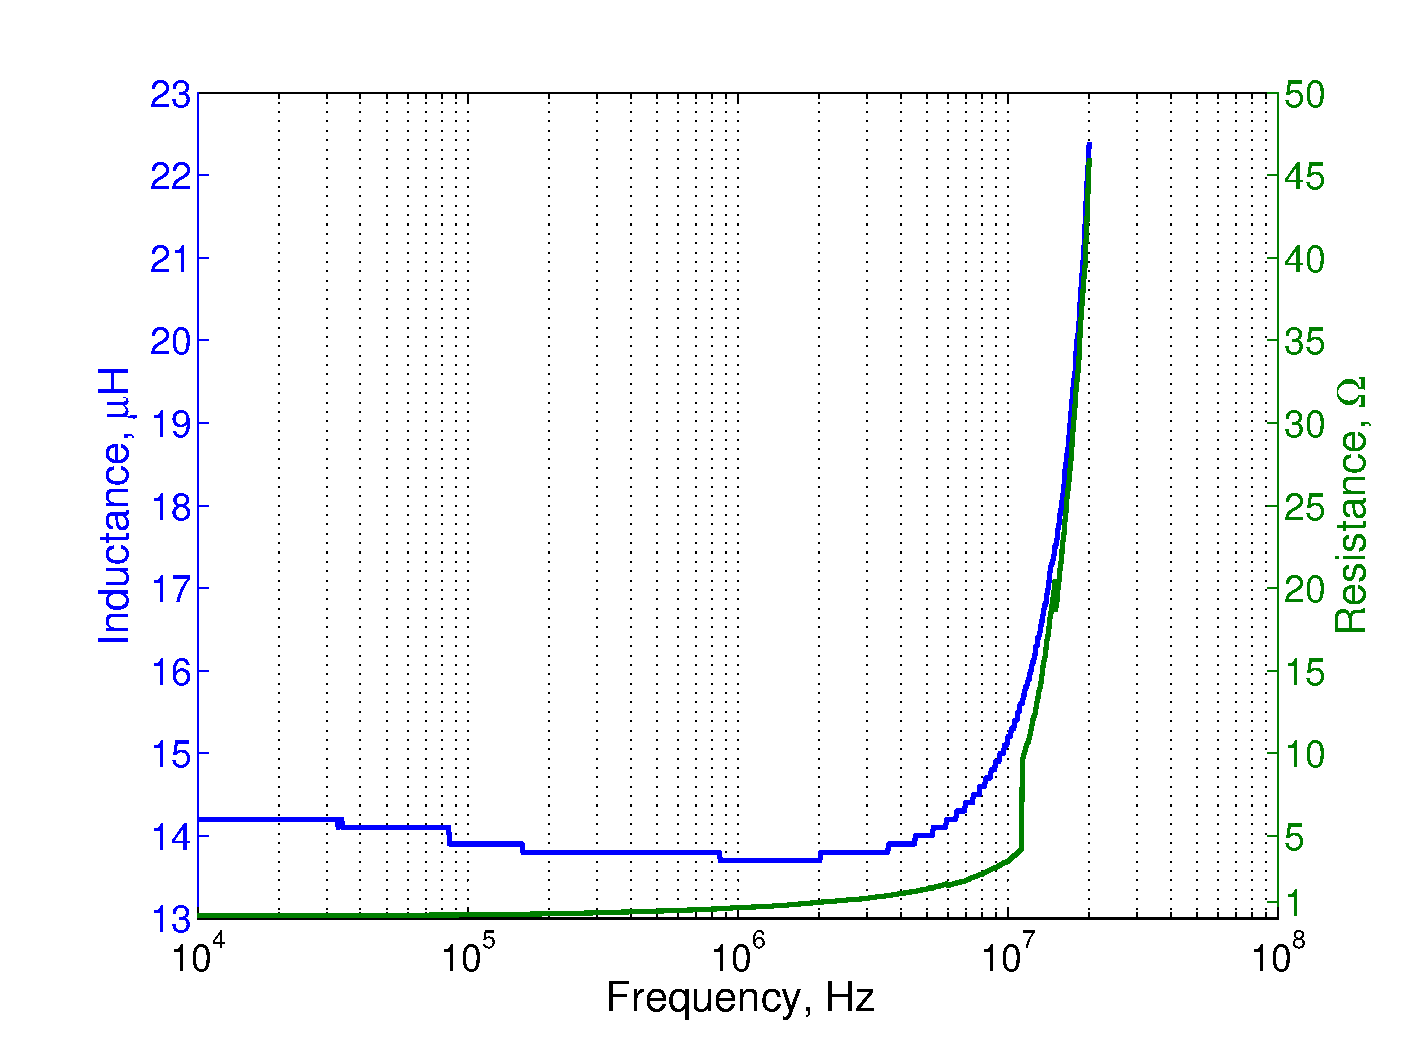
\includegraphics{./images/brx}\label{F:LRbrx}}
\subfigure[Model C transmitter]
	{\includegraphics{./images/ctx}\label{F:LRctx}} 
\subfigure[Model C receiver]
	{\includegraphics{./images/crx}\label{F:LRcrx}}
\end{subfigmatrix}
\end{figure}

\begin{figure}[H]
\centering
\begin{subfigmatrix}{2} 
\subfigure[Model D1] 
	{\includegraphics{./images/d1}\label{F:LRd1}} 
\subfigure[Model D2]
	{\includegraphics{./images/d2}\label{F:LRd2}}
\end{subfigmatrix}
\caption{Inductance and resistance w.r.t. frequency}
\label{F:LRvsF}
\end{figure}


\section{Quality Factor}

\begin{figure}[htb]
\centering
\includegraphics[width=1\textwidth]{./images/QFactorall}
\caption{Experimental quality factor}
\label{F:QFactorAll}
\end{figure}






%%%%%%%%%%%%%%%%%%%%%%%%%%%%%%%%%%%%%%%%%%%%%%%%%%%%
%%%%%%%%%%%%%%%%%%%%%%%%%%%%%%%%%%%%%%%%%%%%%%%%%%%%
\chapter{Circuit Schematics}

\section{Voltage Regulator}\label{Appendix: DC-DC}

% \begin{figure}[htb]
% 	\begin{center}
% 		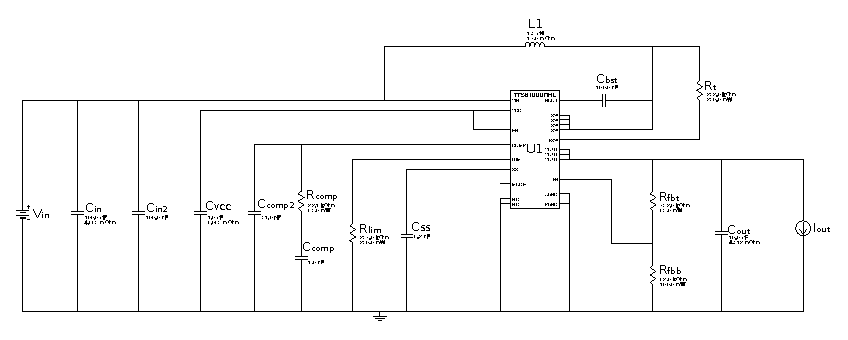
\includegraphics[width=1.05\textwidth]{./images/TPS61088}
% 	\caption{TPS61088 design circuit}
% 	\end{center}
% \end{figure}

\begin{figure}[htb]
	\begin{center}
		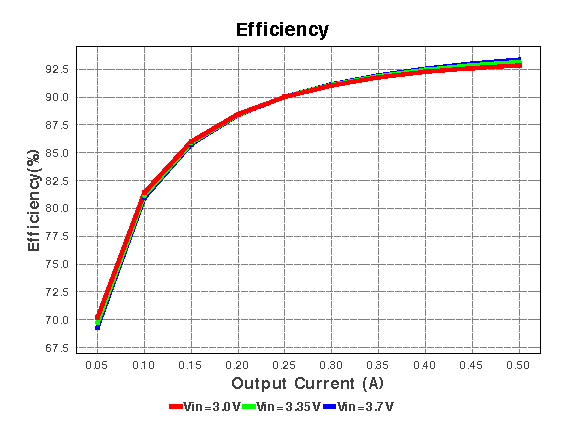
\includegraphics[width=0.8\textwidth]{./images/Efficiency_TPS61088}
	\caption{Efficiency w.r.t. output current}
	\end{center}
\end{figure}

\section{Power Driver}\label{Appendix: powerDriver}
% \begin{figure}[H]
% 	\begin{center}
% 		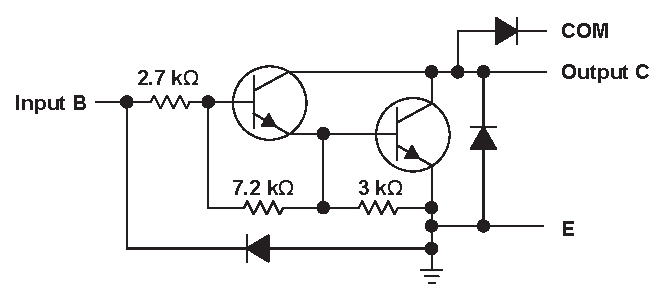
\includegraphics[width=0.8\textwidth]{./images/ULN2803A}
% 	\caption{Functional block diagram of the ULN2803A}
% 	\end{center}
% \end{figure}

\begin{figure}[H]
\centering
\begin{subfigmatrix}{2} 
\hspace*{\fill}%
\subfigure[Functional block diagram] 
	{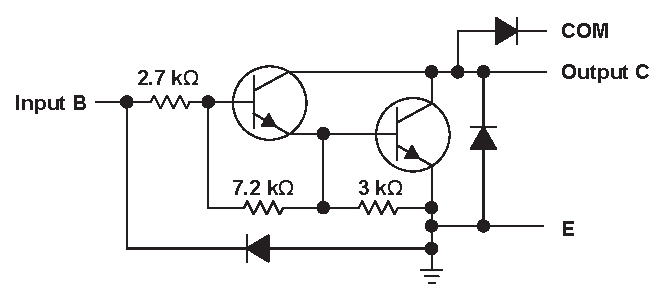
\includegraphics[width=3.0in]{./images/ULN2803A}}\hfill
\subfigure[Top view]
	{
\includegraphics[width=1.0in]{./images/ulnpins}}
\hspace*{\fill}%
\end{subfigmatrix}
\caption{ULN2803 Darlington driver}
\end{figure}


\section{Transmitter}

\begin{figure}[H]
\begin{center}
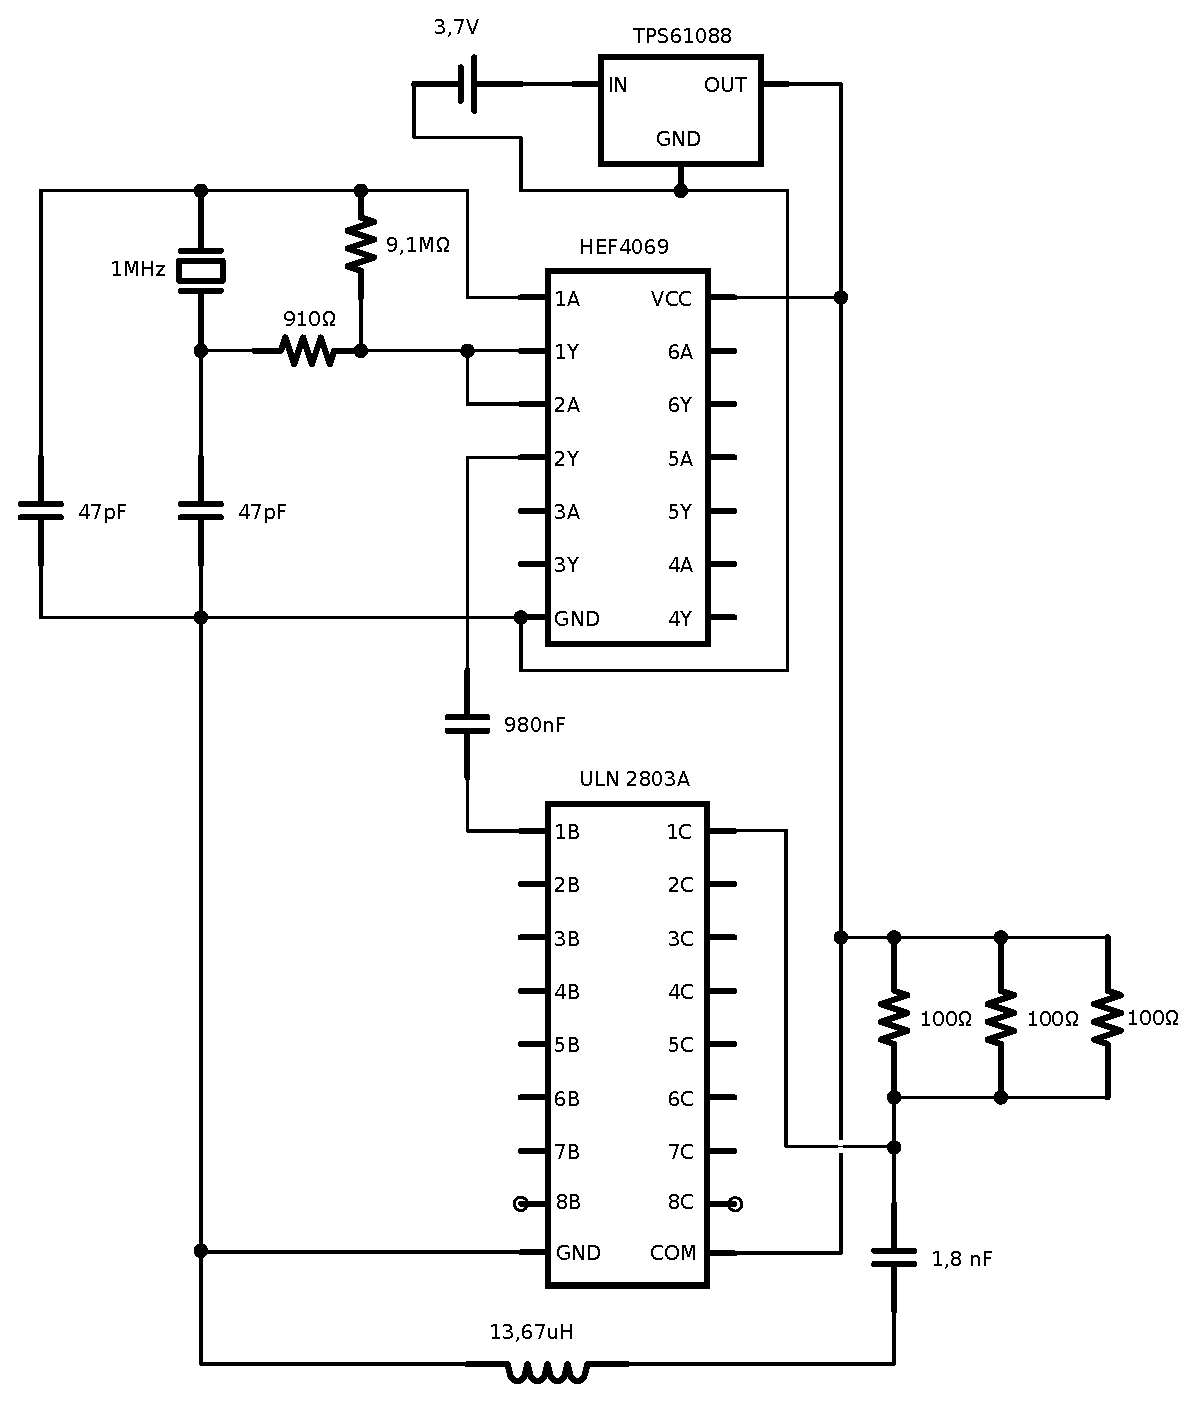
\includegraphics[width=1\textwidth]{./images/circuitv5}
\caption{Transmitter circuit schematic}
% \label{F:contourLines}
\end{center}
\end{figure}

\section{Receiver}
\begin{figure}[H]
\begin{center}
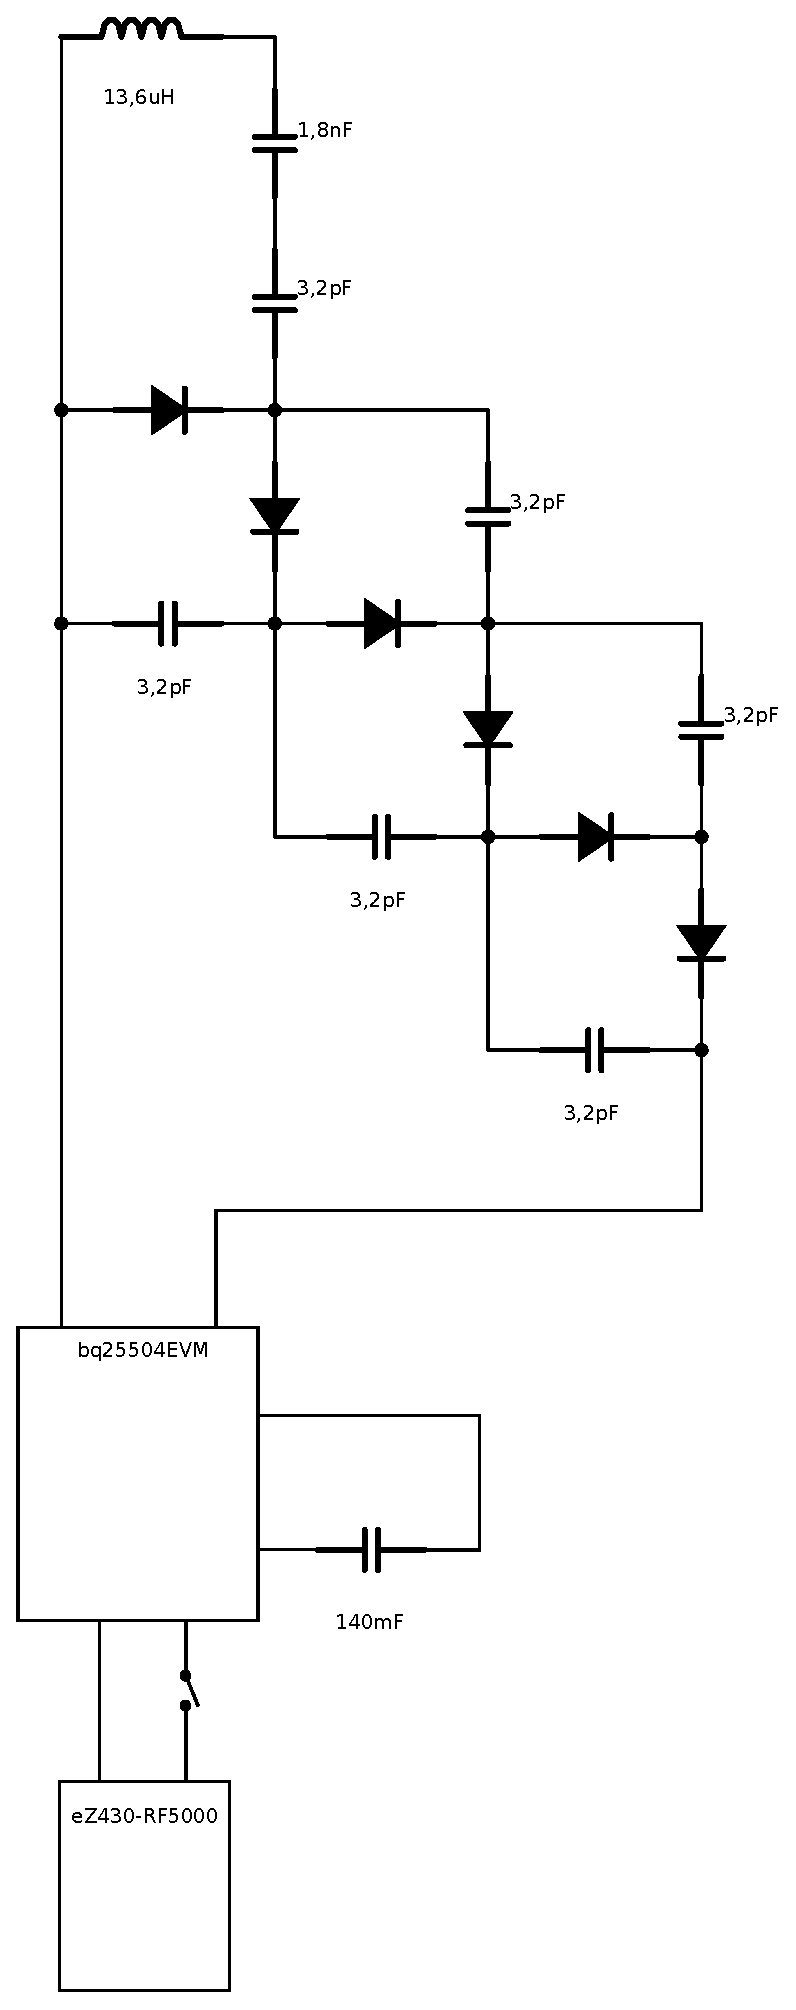
\includegraphics[width=0.55\textwidth]{./images/ReceiverSchematic}
\caption{Receiver circuit schematic}
% \label{F:contourLines}
\end{center}
\end{figure}









\chapter{Experimental Results} \label{Appendix: experimental}

\section{Model A}

\begin{figure}[h]
\centering
\begin{subfigmatrix}{2} 
\subfigure[f = 0.7 MHz]
{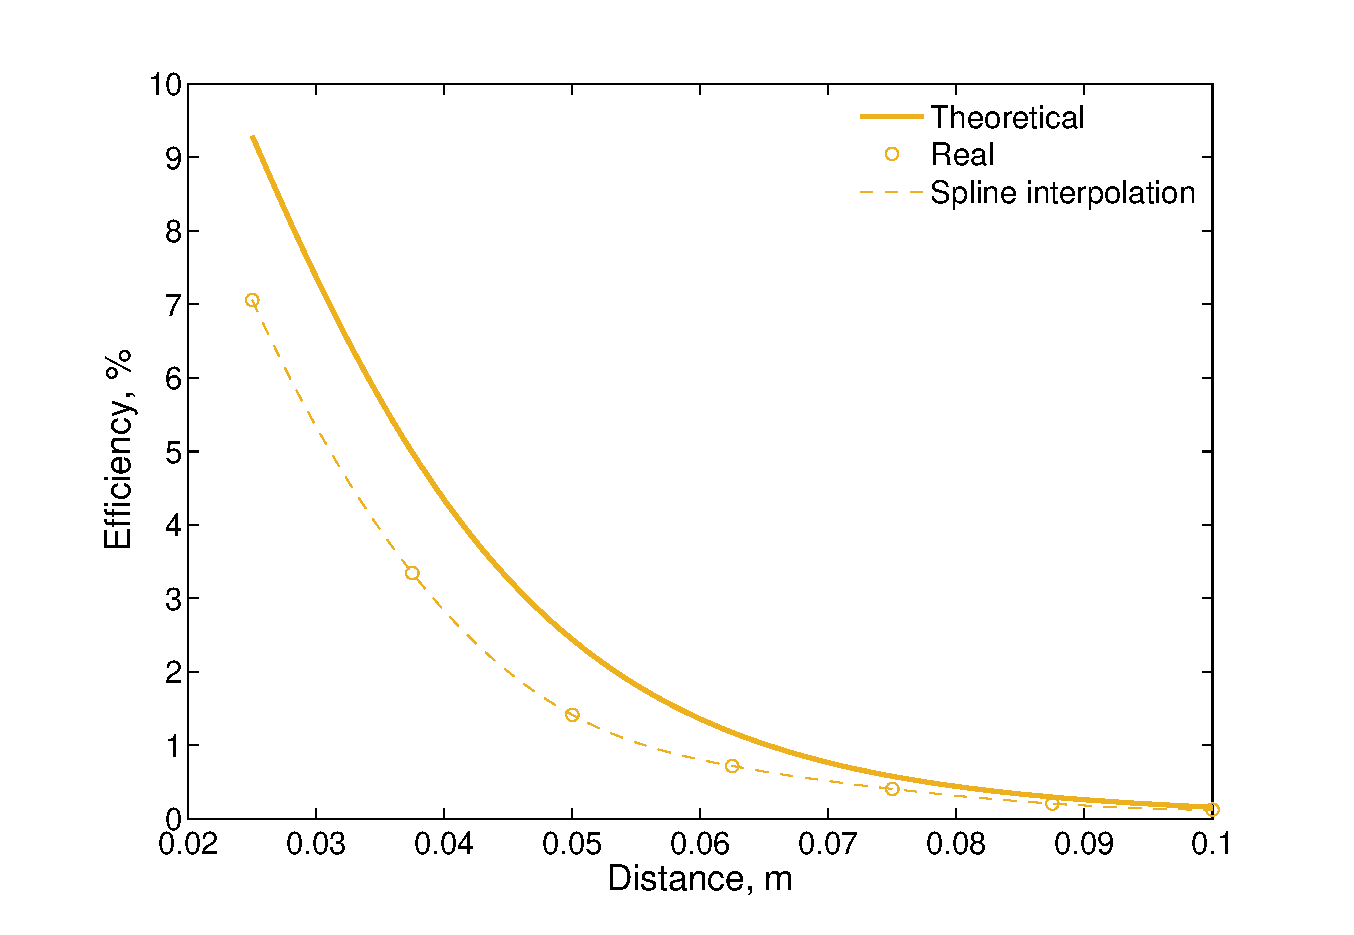
\includegraphics{./images/ModeloS_A_2_eff}}
\subfigure[f = 1 MHz]
{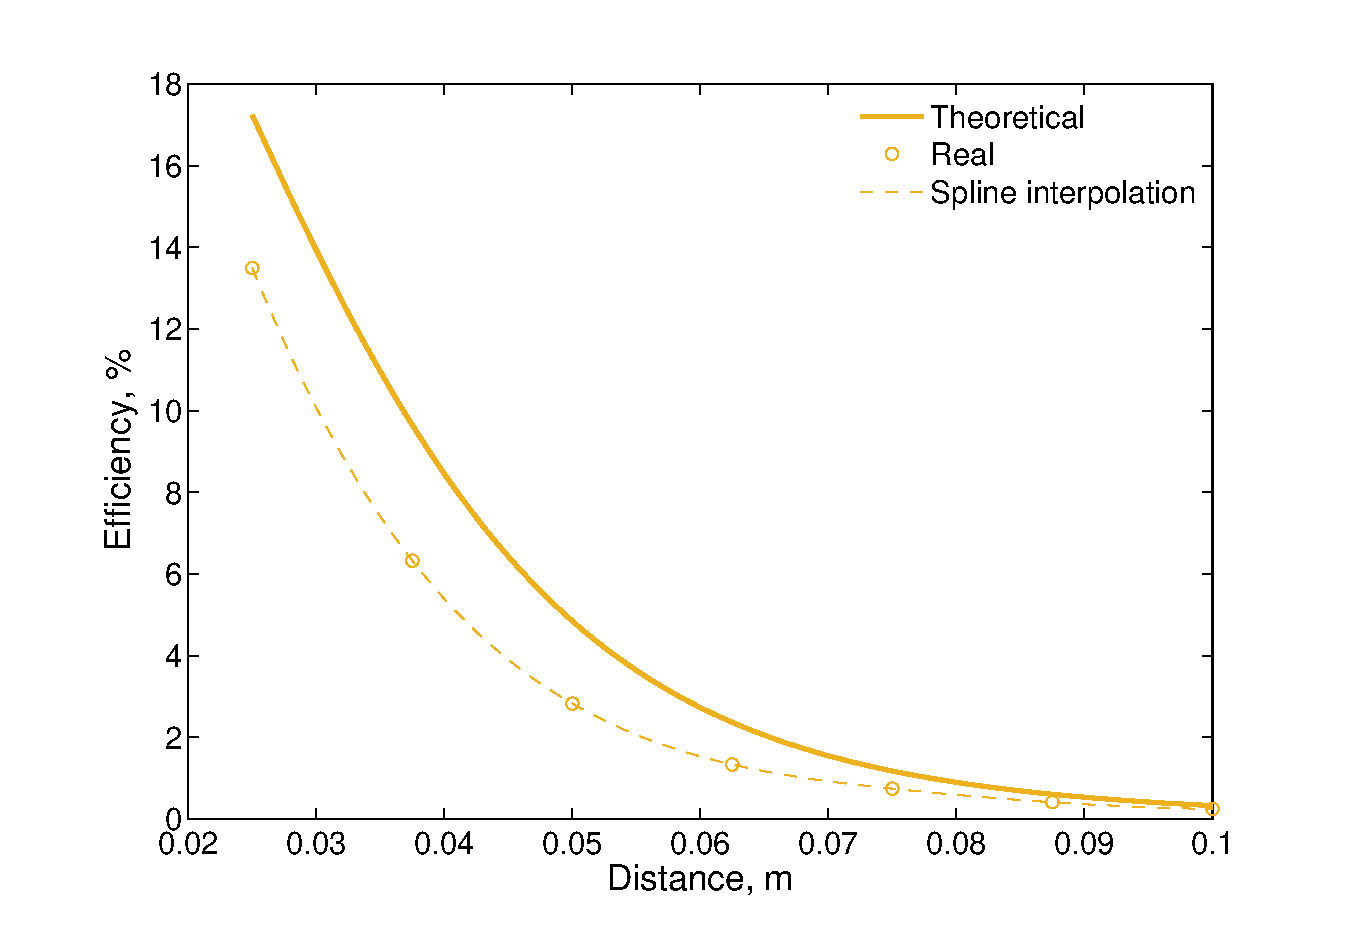
\includegraphics{./images/ModeloS_A_1_eff}}
\end{subfigmatrix}
\end{figure}
% \\[1pt]
\begin{figure}[H]
\centering
\begin{subfigmatrix}{1} 
\subfigure[f = 2 MHz] 
{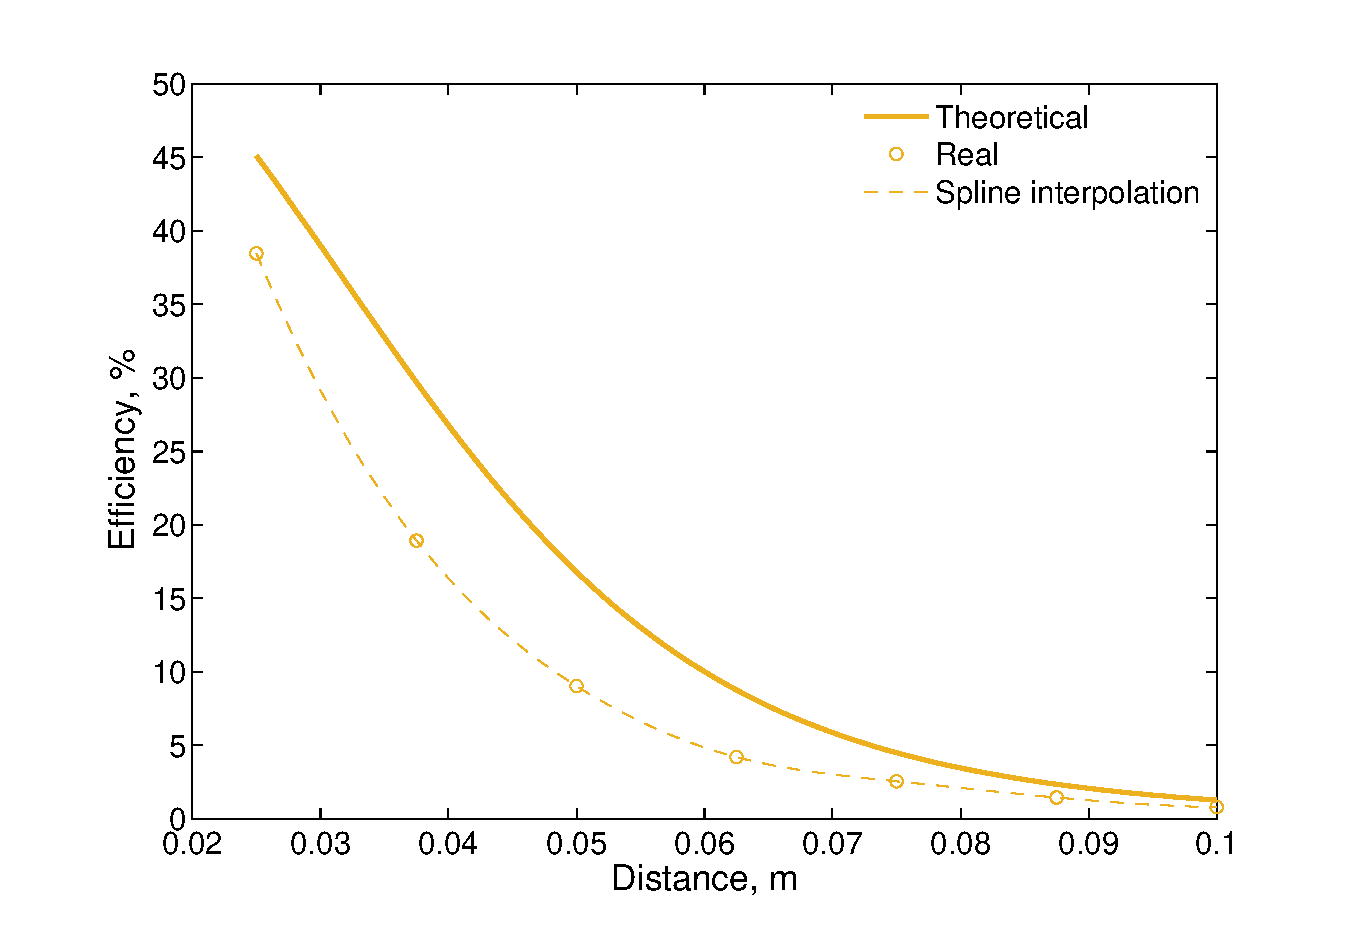
\includegraphics[width=0.5\textwidth]{./images/ModeloS_A_3_eff}}
\end{subfigmatrix}
\caption{Efficiency w.r.t. distance for SS topology}
\end{figure}

%%%%%%%%%%%%%%%%%%%%%%%%%%%%%%%%%%%%%%%%%%%%%%%%

\begin{figure}[h]
\centering
\begin{subfigmatrix}{2} 
\subfigure[f = 0.7 MHz]
{\includegraphics{./images/ModeloS_A_2_pout}}
\subfigure[f = 1 MHz]
{\includegraphics{./images/ModeloS_A_1_pout}}
\end{subfigmatrix}
\end{figure}
\begin{figure}[H]
\centering
\begin{subfigmatrix}{1} 
\subfigure[f = 2 MHz] 
{\includegraphics[width=0.5\textwidth]{./images/ModeloS_A_3_pout}}
\end{subfigmatrix}
\caption{Output power w.r.t. distance for SS topology}
\end{figure}

%%%%%%%%%%%%%%%%%%%%%%%%%%%%%%%%%%%%%%%%%%%%%%%%

\begin{figure}[h]
\centering
\begin{subfigmatrix}{2} 
\subfigure[f = 0.7 MHz]
{\includegraphics{./images/ModeloP_A_2_eff}}
\subfigure[f = 1 MHz]
{\includegraphics{./images/ModeloP_A_1_eff}}
\end{subfigmatrix}
\end{figure}
\begin{figure}[H]
\centering
\begin{subfigmatrix}{1} 
\subfigure[f = 2 MHz] 
{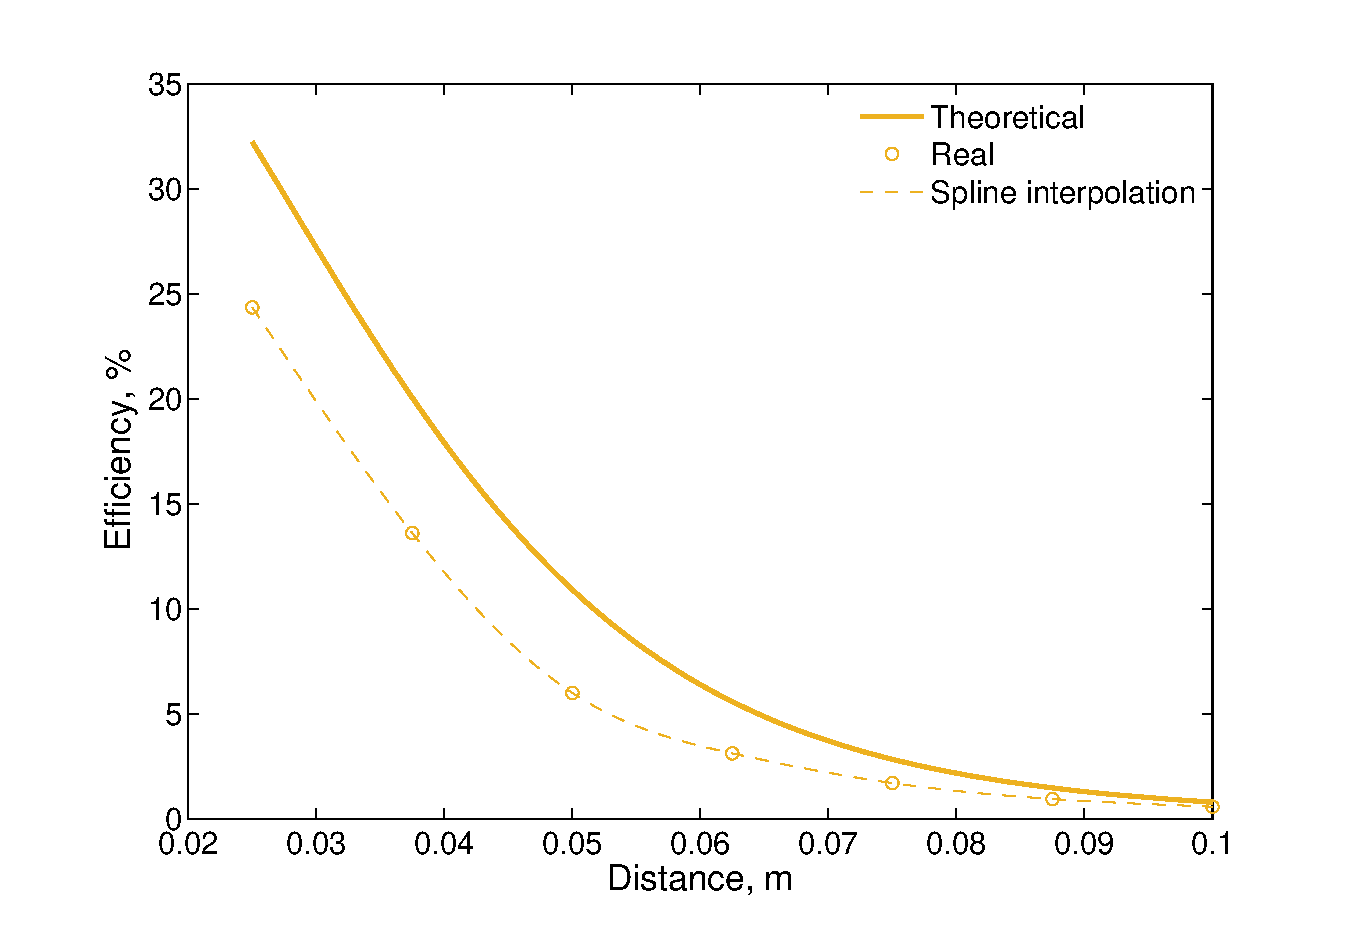
\includegraphics[width=0.5\textwidth]{./images/ModeloP_A_3_eff}}
\end{subfigmatrix}
\caption{Efficiency w.r.t. distance for SP topology}
\end{figure}

%%%%%%%%%%%%%%%%%%%%%%%%%%%%%%%%%%%%%%%%%%%%%%%%

\begin{figure}[h]
\centering
\begin{subfigmatrix}{2} 
\subfigure[f = 0.7 MHz]
{\includegraphics{./images/ModeloP_A_2_pout}}
\subfigure[f = 1 MHz]
{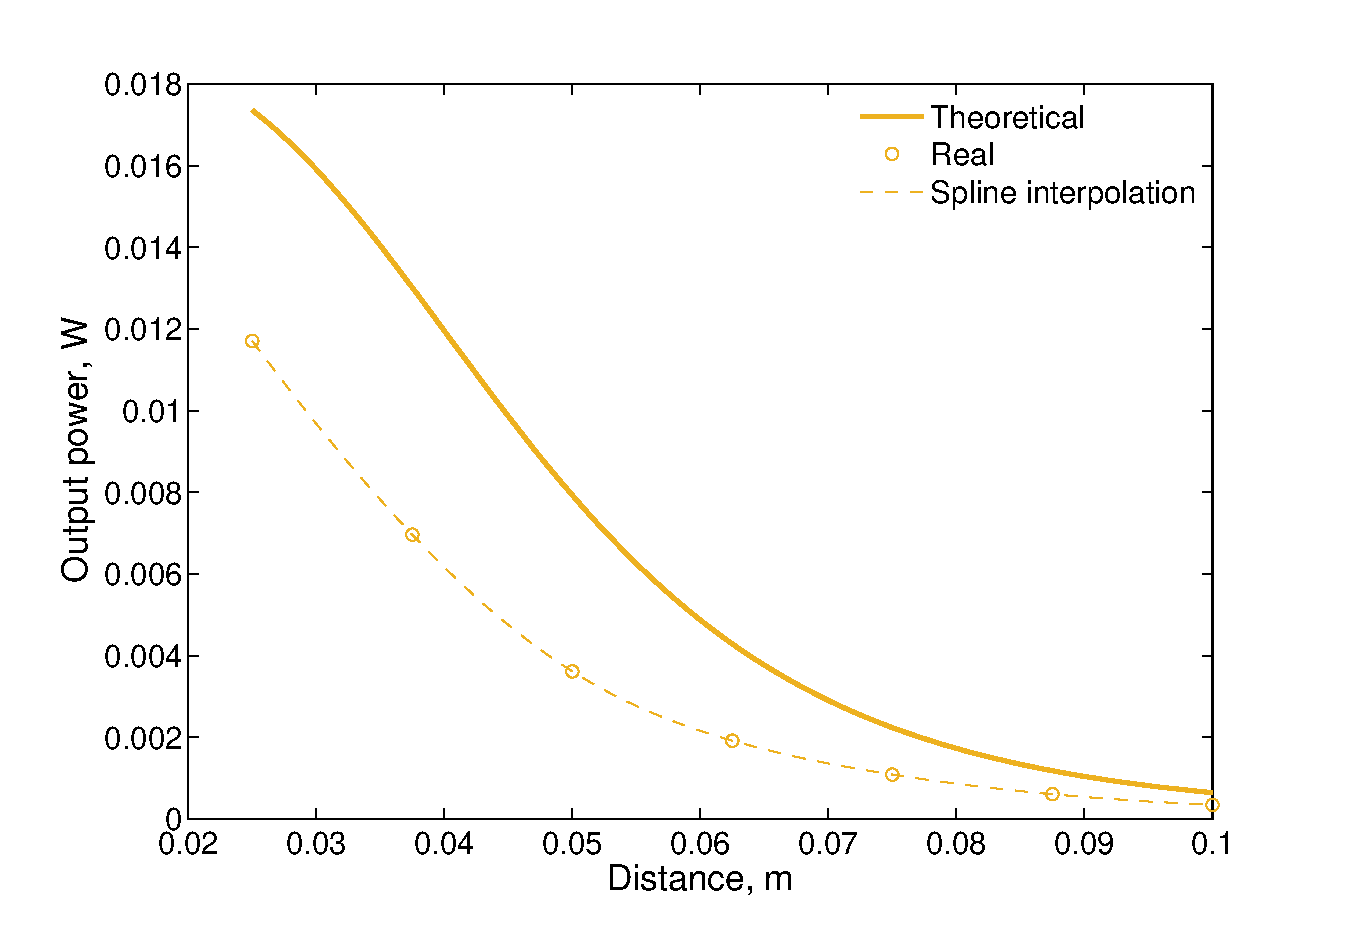
\includegraphics{./images/ModeloP_A_1_pout}}
\end{subfigmatrix}
\end{figure}
\begin{figure}[H]
\centering
\begin{subfigmatrix}{1} 
\subfigure[f = 2 MHz] 
{\includegraphics[width=0.5\textwidth]{./images/ModeloP_A_3_pout}}
\end{subfigmatrix}
\caption{Output power w.r.t. distance for SP topology}
\end{figure}

%%%%%%%%%%%%%%%%%%%%%%%%%%%%%%%%%%%%%%%%%%%%%%%%

\begin{figure}[h]
\centering
\begin{subfigmatrix}{2} 
\subfigure[f = 0.7 MHz]
{\includegraphics{./images/ModeloS_A_ZL_2_eff}}
\subfigure[f = 1 MHz]
{\includegraphics{./images/ModeloS_A_ZL_1_eff}}
\end{subfigmatrix}
\end{figure}
\begin{figure}[H]
\centering
\begin{subfigmatrix}{1} 
\subfigure[f = 2 MHz] 
{\includegraphics[width=0.5\textwidth]{./images/ModeloS_A_ZL_3_eff}}
\end{subfigmatrix}
\caption{Efficiency w.r.t. load resistance for SS topology}
\end{figure}

%%%%%%%%%%%%%%%%%%%%%%%%%%%%%%%%%%%%%%%%%%%%%%%%

\begin{figure}[h]
\centering
\begin{subfigmatrix}{2} 
\subfigure[f = 0.7 MHz]
{\includegraphics{./images/ModeloS_A_ZL_2_pout}}
\subfigure[f = 1 MHz]
{\includegraphics{./images/ModeloS_A_ZL_1_pout}}
\end{subfigmatrix}
\end{figure}
\begin{figure}[H]
\centering
\begin{subfigmatrix}{1} 
\subfigure[f = 2 MHz] 
{\includegraphics[width=0.5\textwidth]{./images/ModeloS_A_ZL_3_pout}}
\end{subfigmatrix}
\caption{Output power w.r.t. load resistance for SS topology}
\end{figure}

%%%%%%%%%%%%%%%%%%%%%%%%%%%%%%%%%%%%%%%%%%%%%%%%

\begin{figure}[h]
\centering
\begin{subfigmatrix}{2} 
\subfigure[f = 0.7 MHz]
{\includegraphics{./images/ModeloP_A_ZL_2_eff}}
\subfigure[f = 1 MHz]
{\includegraphics{./images/ModeloP_A_ZL_1_eff}}
\end{subfigmatrix}
\end{figure}
\begin{figure}[H]
\centering
\begin{subfigmatrix}{1} 
\subfigure[f = 2 MHz] 
{\includegraphics[width=0.5\textwidth]{./images/ModeloP_A_ZL_3_eff}}
\end{subfigmatrix}
\caption{Efficiency w.r.t. load resistance for SP topology}
\end{figure}

%%%%%%%%%%%%%%%%%%%%%%%%%%%%%%%%%%%%%%%%%%%%%%%%

\begin{figure}[h]
\centering
\begin{subfigmatrix}{2} 
\subfigure[f = 0.7 MHz]
{\includegraphics{./images/ModeloP_A_ZL_2_pout}}
\subfigure[f = 1 MHz]
{\includegraphics{./images/ModeloP_A_ZL_1_pout}}
\end{subfigmatrix}
\end{figure}
\begin{figure}[H]
\centering
\begin{subfigmatrix}{1} 
\subfigure[f = 2 MHz] 
{\includegraphics[width=0.5\textwidth]{./images/ModeloP_A_ZL_3_pout}}
\end{subfigmatrix}
\caption{Output power w.r.t. load resistance for SP topology}
\end{figure}

%%%%%%%%%%%%%%%%%%%%%%%%%%%%%%%%%%%%%%%%%%%%%%%%
%%%%%%%%%%%%%%%%%%%%%%%%%%%%%%%%%%%%%%%%%%%%%%%%
%%%%%%%%%%%%%%%%%%%%%%%%%%%%%%%%%%%%%%%%%%%%%%%%

\section{Model B}

\begin{figure}[h]
\centering
\begin{subfigmatrix}{2} 
\subfigure[f = 0.7 MHz]
{\includegraphics{./images/ModeloS_B_2_eff}}
\subfigure[f = 1 MHz]
{\includegraphics{./images/ModeloS_B_1_eff}}
\end{subfigmatrix}
\end{figure}
% \\[1pt]
\begin{figure}[H]
\centering
\begin{subfigmatrix}{1} 
\subfigure[f = 2 MHz] 
{\includegraphics[width=0.5\textwidth]{./images/ModeloS_B_3_eff}}
\end{subfigmatrix}
\caption{Efficiency w.r.t. distance for SS topology}
\end{figure}

%%%%%%%%%%%%%%%%%%%%%%%%%%%%%%%%%%%%%%%%%%%%%%%%

\begin{figure}[h]
\centering
\begin{subfigmatrix}{2} 
\subfigure[f = 0.7 MHz]
{\includegraphics{./images/ModeloS_B_2_pout}}
\subfigure[f = 1 MHz]
{\includegraphics{./images/ModeloS_B_1_pout}}
\end{subfigmatrix}
\end{figure}
\begin{figure}[H]
\centering
\begin{subfigmatrix}{1} 
\subfigure[f = 2 MHz] 
{\includegraphics[width=0.5\textwidth]{./images/ModeloS_B_3_pout}}
\end{subfigmatrix}
\caption{Output power w.r.t. distance for SS topology}
\end{figure}

%%%%%%%%%%%%%%%%%%%%%%%%%%%%%%%%%%%%%%%%%%%%%%%%

\begin{figure}[h]
\centering
\begin{subfigmatrix}{2} 
\subfigure[f = 0.7 MHz]
{\includegraphics{./images/ModeloP_B_2_eff}}
\subfigure[f = 1 MHz]
{\includegraphics{./images/ModeloP_B_1_eff}}
\end{subfigmatrix}
\end{figure}
\begin{figure}[H]
\centering
\begin{subfigmatrix}{1} 
\subfigure[f = 2 MHz] 
{\includegraphics[width=0.5\textwidth]{./images/ModeloP_B_3_eff}}
\end{subfigmatrix}
\caption{Efficiency w.r.t. distance for SP topology}
\end{figure}

%%%%%%%%%%%%%%%%%%%%%%%%%%%%%%%%%%%%%%%%%%%%%%%%

\begin{figure}[h]
\centering
\begin{subfigmatrix}{2} 
\subfigure[f = 0.7 MHz]
{\includegraphics{./images/ModeloP_B_2_pout}}
\subfigure[f = 1 MHz]
{\includegraphics{./images/ModeloP_B_1_pout}}
\end{subfigmatrix}
\end{figure}
\begin{figure}[H]
\centering
\begin{subfigmatrix}{1} 
\subfigure[f = 2 MHz] 
{\includegraphics[width=0.5\textwidth]{./images/ModeloP_B_3_pout}}
\end{subfigmatrix}
\caption{Output power w.r.t. distance for SP topology}
\end{figure}

%%%%%%%%%%%%%%%%%%%%%%%%%%%%%%%%%%%%%%%%%%%%%%%%

\begin{figure}[h]
\centering
\begin{subfigmatrix}{2} 
\subfigure[f = 0.7 MHz]
{\includegraphics{./images/ModeloS_B_ZL_2_eff}}
\subfigure[f = 1 MHz]
{\includegraphics{./images/ModeloS_B_ZL_1_eff}}
\end{subfigmatrix}
\end{figure}
\begin{figure}[H]
\centering
\begin{subfigmatrix}{1} 
\subfigure[f = 2 MHz] 
{\includegraphics[width=0.5\textwidth]{./images/ModeloS_B_ZL_3_eff}}
\end{subfigmatrix}
\caption{Efficiency w.r.t. load resistance for SS topology}
\end{figure}

%%%%%%%%%%%%%%%%%%%%%%%%%%%%%%%%%%%%%%%%%%%%%%%%

\begin{figure}[h]
\centering
\begin{subfigmatrix}{2} 
\subfigure[f = 0.7 MHz]
{\includegraphics{./images/ModeloS_B_ZL_2_pout}}
\subfigure[f = 1 MHz]
{\includegraphics{./images/ModeloS_B_ZL_1_pout}}
\end{subfigmatrix}
\end{figure}
\begin{figure}[H]
\centering
\begin{subfigmatrix}{1} 
\subfigure[f = 2 MHz] 
{\includegraphics[width=0.5\textwidth]{./images/ModeloS_B_ZL_3_pout}}
\end{subfigmatrix}
\caption{Output power w.r.t. load resistance for SS topology}
\end{figure}

%%%%%%%%%%%%%%%%%%%%%%%%%%%%%%%%%%%%%%%%%%%%%%%%

\begin{figure}[h]
\centering
\begin{subfigmatrix}{2} 
\subfigure[f = 0.7 MHz]
{\includegraphics{./images/ModeloP_B_ZL_2_eff}}
\subfigure[f = 1 MHz]
{\includegraphics{./images/ModeloP_B_ZL_1_eff}}
\end{subfigmatrix}
\end{figure}
\begin{figure}[H]
\centering
\begin{subfigmatrix}{1} 
\subfigure[f = 2 MHz] 
{\includegraphics[width=0.5\textwidth]{./images/ModeloP_B_ZL_3_eff}}
\end{subfigmatrix}
\caption{Efficiency w.r.t. load resistance for SP topology}
\end{figure}

%%%%%%%%%%%%%%%%%%%%%%%%%%%%%%%%%%%%%%%%%%%%%%%%

\begin{figure}[h]
\centering
\begin{subfigmatrix}{2} 
\subfigure[f = 0.7 MHz]
{\includegraphics{./images/ModeloP_B_ZL_2_pout}}
\subfigure[f = 1 MHz]
{\includegraphics{./images/ModeloP_B_ZL_1_pout}}
\end{subfigmatrix}
\end{figure}
\begin{figure}[H]
\centering
\begin{subfigmatrix}{1} 
\subfigure[f = 2 MHz] 
{\includegraphics[width=0.5\textwidth]{./images/ModeloP_B_ZL_3_pout}}
\end{subfigmatrix}
\caption{Output power w.r.t. load resistance for SP topology}
\end{figure}

%%%%%%%%%%%%%%%%%%%%%%%%%%%%%%%%%%%%%%%%%%%%%%%%
%%%%%%%%%%%%%%%%%%%%%%%%%%%%%%%%%%%%%%%%%%%%%%%%
%%%%%%%%%%%%%%%%%%%%%%%%%%%%%%%%%%%%%%%%%%%%%%%%

\section{Model C}

\begin{figure}[h]
\centering
\begin{subfigmatrix}{2} 
\subfigure[f = 0.7 MHz]
{\includegraphics{./images/ModeloS_C_2_eff}}
\subfigure[f = 1 MHz]
{\includegraphics{./images/ModeloS_C_1_eff}}
\end{subfigmatrix}
\end{figure}
% \\[1pt]
\begin{figure}[H]
\centering
\begin{subfigmatrix}{1} 
\subfigure[f = 2 MHz] 
{\includegraphics[width=0.5\textwidth]{./images/ModeloS_C_3_eff}}
\end{subfigmatrix}
\caption{Efficiency w.r.t. distance for SS topology}
\end{figure}

%%%%%%%%%%%%%%%%%%%%%%%%%%%%%%%%%%%%%%%%%%%%%%%%

\begin{figure}[h]
\centering
\begin{subfigmatrix}{2} 
\subfigure[f = 0.7 MHz]
{\includegraphics{./images/ModeloS_C_2_pout}}
\subfigure[f = 1 MHz]
{\includegraphics{./images/ModeloS_C_1_pout}}
\end{subfigmatrix}
\end{figure}
\begin{figure}[H]
\centering
\begin{subfigmatrix}{1} 
\subfigure[f = 2 MHz] 
{\includegraphics[width=0.5\textwidth]{./images/ModeloS_C_3_pout}}
\end{subfigmatrix}
\caption{Output power w.r.t. distance for SS topology}
\end{figure}

%%%%%%%%%%%%%%%%%%%%%%%%%%%%%%%%%%%%%%%%%%%%%%%%

\begin{figure}[h]
\centering
\begin{subfigmatrix}{2} 
\subfigure[f = 0.7 MHz]
{\includegraphics{./images/ModeloP_C_2_eff}}
\subfigure[f = 1 MHz]
{\includegraphics{./images/ModeloP_C_1_eff}}
\end{subfigmatrix}
\end{figure}
\begin{figure}[H]
\centering
\begin{subfigmatrix}{1} 
\subfigure[f = 2 MHz] 
{\includegraphics[width=0.5\textwidth]{./images/ModeloP_C_3_eff}}
\end{subfigmatrix}
\caption{Efficiency w.r.t. distance for SP topology}
\end{figure}

%%%%%%%%%%%%%%%%%%%%%%%%%%%%%%%%%%%%%%%%%%%%%%%%

\begin{figure}[h]
\centering
\begin{subfigmatrix}{2} 
\subfigure[f = 0.7 MHz]
{\includegraphics{./images/ModeloP_C_2_pout}}
\subfigure[f = 1 MHz]
{\includegraphics{./images/ModeloP_C_1_pout}}
\end{subfigmatrix}
\end{figure}
\begin{figure}[H]
\centering
\begin{subfigmatrix}{1} 
\subfigure[f = 2 MHz] 
{\includegraphics[width=0.5\textwidth]{./images/ModeloP_C_3_pout}}
\end{subfigmatrix}
\caption{Output power w.r.t. distance for SP topology}
\end{figure}

%%%%%%%%%%%%%%%%%%%%%%%%%%%%%%%%%%%%%%%%%%%%%%%%
%%%%%%%%%%%%%%%%%%%%%%%%%%%%%%%%%%%%%%%%%%%%%%%%
\begin{figure}[h]
\centering
\begin{subfigmatrix}{2} 
\subfigure[f = 0.7 MHz]
{\includegraphics{./images/ModeloS_C_ZL_2_eff}}
\subfigure[f = 1 MHz]
{\includegraphics{./images/ModeloS_C_ZL_1_eff}}
\end{subfigmatrix}
\end{figure}
\begin{figure}[H]
\centering
\begin{subfigmatrix}{1} 
\subfigure[f = 2 MHz] 
{\includegraphics[width=0.5\textwidth]{./images/ModeloS_C_ZL_3_eff}}
\end{subfigmatrix}
\caption{Efficiency w.r.t. load resistance for SS topology}
\end{figure}

%%%%%%%%%%%%%%%%%%%%%%%%%%%%%%%%%%%%%%%%%%%%%%%%

\begin{figure}[h]
\centering
\begin{subfigmatrix}{2} 
\subfigure[f = 0.7 MHz]
{\includegraphics{./images/ModeloS_C_ZL_2_pout}}
\subfigure[f = 1 MHz]
{\includegraphics{./images/ModeloS_C_ZL_1_pout}}
\end{subfigmatrix}
\end{figure}
\begin{figure}[H]
\centering
\begin{subfigmatrix}{1} 
\subfigure[f = 2 MHz] 
{\includegraphics[width=0.5\textwidth]{./images/ModeloS_C_ZL_3_pout}}
\end{subfigmatrix}
\caption{Output power w.r.t. load resistance for SS topology}
\end{figure}

%%%%%%%%%%%%%%%%%%%%%%%%%%%%%%%%%%%%%%%%%%%%%%%%

\begin{figure}[h]
\centering
\begin{subfigmatrix}{2} 
\subfigure[f = 0.7 MHz]
{\includegraphics{./images/ModeloP_C_ZL_2_eff}}
\subfigure[f = 1 MHz]
{\includegraphics{./images/ModeloP_C_ZL_1_eff}}
\end{subfigmatrix}
\end{figure}
\begin{figure}[H]
\centering
\begin{subfigmatrix}{1} 
\subfigure[f = 2 MHz] 
{\includegraphics[width=0.5\textwidth]{./images/ModeloP_C_ZL_3_eff}}
\end{subfigmatrix}
\caption{Efficiency w.r.t. load resistance for SP topology}
\end{figure}

%%%%%%%%%%%%%%%%%%%%%%%%%%%%%%%%%%%%%%%%%%%%%%%%

\begin{figure}[h]
\centering
\begin{subfigmatrix}{2} 
\subfigure[f = 0.7 MHz]
{\includegraphics{./images/ModeloP_C_ZL_2_pout}}
\subfigure[f = 1 MHz]
{\includegraphics{./images/ModeloP_C_ZL_1_pout}}
\end{subfigmatrix}
\end{figure}
\begin{figure}[H]
\centering
\begin{subfigmatrix}{1} 
\subfigure[f = 2 MHz] 
{\includegraphics[width=0.5\textwidth]{./images/ModeloP_C_ZL_3_pout}}
\end{subfigmatrix}
\caption{Output power w.r.t. load resistance for SP topology}
\end{figure}

%%%%%%%%%%%%%%%%%%%%%%%%%%%%%%%%%%%%%%%%%%%%%%%%
%%%%%%%%%%%%%%%%%%%%%%%%%%%%%%%%%%%%%%%%%%%%%%%%
%%%%%%%%%%%%%%%%%%%%%%%%%%%%%%%%%%%%%%%%%%%%%%%%
\section{Output power for models D1 and D2}\label{D1D2}
This plots demonstrate that a bigger receiver coil diameter is preferred upon a bigger transmitter coil diameter. This is stated at Section \ref{subsec:geo}
\begin{figure}[H]
\centering
\begin{subfigmatrix}{2} 
\subfigure[D1 (Tx) / D2 (Rx)]
{\includegraphics{./images/D12}}
\subfigure[D2 (Tx) / D1 (Rx)]
{\includegraphics{./images/D21}}
\end{subfigmatrix}
\caption{Experimental demonstration of the output power depending on the coil receiver radius}
\end{figure}







\chapter{Programming Code}
Along this project, the plots and the mathematical model have been perfomed using \textit{MATLAB}. Some important codes are shown below. 


%% MATLAB example
% \begin{lstlisting}
% function y = myfun(aa, sigma, options)
% \end{lstlisting}

\lstinputlisting{./matlab/ExperimentalCoils.m}
\lstinputlisting{./matlab/FourTopologies.m}
\lstinputlisting{./matlab/SStopologyModel.m}
\lstinputlisting{./matlab/SPtopologyModel.m}
\lstinputlisting{./matlab/AC_Resistance.m}

\includepdf[pages={1}]{./images/MotorMount1.pdf}
\includepdf[pages={1}]{./images/BQ25504datasheet.pdf}
\includepdf[pages={2}]{./images/BQ25504datasheet.pdf}
\includepdf[pages={3}]{./images/BQ25504datasheet.pdf}
\includepdf[pages={4}]{./images/BQ25504datasheet.pdf}
\includepdf[pages={5}]{./images/slau227f.pdf}
\includepdf[pages={8}]{./images/slau227f.pdf}




%%%%%%%%%%%%%%%%%%%%%%%%%%%%%%%%%%%%%%%%%%%%%%%%%%%%%%%%%%%%%%%%%%%%%%%%%%
%%%%%%%%%%%%%%%%%%%%%%%%%%%%%%%%%%%%%%%%%%%%%%%%%%%%%%%%%%%%%%%%%%%%%%%%%%
%%%%%%%%%%%%%%%%%%%%%%%%%%%%%%%%%%%%%%%%%%%%%%%%%%%%%%%%%%%%%%%%%%%%%%%%%%
\end{document}
